\chapter{Đọc thêm 2: Dự đoán Biến động Giá Cổ phiếu từ Cảm xúc Nhà đầu tư trên Stocktwits (Liu, Leu \& Holst)}
\label{ch:M4L3DT2}

% Nguồn: Liu, J.-X., Leu, J.-S., & Holst, S. ``Stock price movement prediction based on Stocktwits investor sentiment using FinBERT and ensemble SVM.'' PeerJ Computer Science, 9:e1403, 2023.
% Phần cần đọc: Toàn bộ bài báo
% Nội dung bắt buộc đọc: được kiểm tra trong mọi bài đánh giá (kể cả Quiz).

\section{Thông tin nguồn}

\begin{itemize}
  \item \textbf{Nguồn:} Liu, Jin-Xian, Jenq-Shiou Leu, and Stefan Holst. \emph{Stock price movement prediction based on Stocktwits investor sentiment using FinBERT and ensemble SVM}. PeerJ Computer Science, 9:e1403, 2023. \url{http://doi.org/10.7717/peerj-cs.1403}
  \item \textbf{Phần cần đọc:} Toàn bộ nội dung
\end{itemize}

\section{Tóm tắt}

Cảm xúc nhà đầu tư đóng vai trò then chốt trong thị trường chứng khoán, và trong những năm gần đây, nhiều nghiên cứu đã nỗ lực dự đoán giá cổ phiếu tương lai bằng cách phân tích cảm xúc thị trường thu thập từ mạng xã hội hoặc tin tức. Nghiên cứu này khảo sát việc sử dụng cảm xúc nhà đầu tư từ mạng xã hội, tập trung vào Stocktwits, một nền tảng mạng xã hội dành cho nhà đầu tư. Tuy nhiên, việc dùng cảm xúc nhà đầu tư trên Stocktwits để dự đoán biến động giá cổ phiếu có thể gặp khó khăn do thiếu dữ liệu cảm xúc do người dùng tự gán nhãn và do hạn chế của các bộ phân loại cảm xúc hiện có, vốn có thể phân loại sai các bình luận trung lập. Để khắc phục những thách thức này, nghiên cứu đề xuất một cách tiếp cận thay thế sử dụng FinBERT, một mô hình ngôn ngữ đã được huấn luyện trước, được thiết kế chuyên biệt để phân tích cảm xúc văn bản tài chính. Nghiên cứu này đề xuất một máy vector hỗ trợ tập hợp (ensemble support vector machine, SVM) nhằm cải thiện độ chính xác của dự đoán biến động giá cổ phiếu. Sau đó, mô hình dự đoán biến động giá tương lai của Quỹ hoán đổi danh mục (Exchange Traded Fund) chỉ số SPDR S\&P 500, sử dụng phương pháp cửa sổ trượt (rolling window) để tránh thiên lệch nhìn trước (look-ahead bias). Thông qua việc so sánh các kỹ thuật khác nhau để tạo ra cảm xúc, kết quả của chúng tôi cho thấy việc sử dụng mô hình FinBERT để phân tích cảm xúc mang lại kết quả tốt nhất, với điểm F1 (F1-score) cao hơn 4 đến 5\% so với các kỹ thuật khác. Ngoài ra, máy vector hỗ trợ tập hợp được đề xuất cải thiện độ chính xác của dự đoán biến động giá cổ phiếu so với máy vector hỗ trợ nguyên bản trong một loạt các thực nghiệm.

\textbf{Chủ đề:} Trí tuệ nhân tạo, Khai phá dữ liệu và Học máy, Khoa học Dữ liệu, Khai phá Văn bản, Phân tích Cảm xúc

\textbf{Từ khóa:} Phân tích cảm xúc, Stocktwits, Dự đoán giá cổ phiếu, Học máy, SVM, SPY, FinBERT, Tài chính

\section{Giới thiệu}

Theo giả thuyết thị trường hiệu quả (efficient market hypothesis, EMH) (Fama, 1970), thị trường chứng khoán được coi là hiệu quả vì người ta giả định rằng tất cả thông tin sẵn có đã được phản ánh vào giá cổ phiếu. Nếu giả định EMH là đúng, thì giả thuyết bước đi ngẫu nhiên (random walk hypothesis) (Fama, 1965) cho rằng tin tức tương lai là ngẫu nhiên và nhà đầu tư không thể sử dụng kiến thức trước đó của mình để tạo ra lợi nhuận vượt trội. Tuy nhiên, nhiều nghiên cứu được thực hiện trong vài thập kỷ qua đã cho thấy rằng việc dự đoán giá thị trường tương lai là khả thi thông qua các kỹ thuật như phân tích cơ bản, phân tích kỹ thuật và phân tích cảm xúc. Trong số đó, dự đoán giá cổ phiếu dựa trên cảm xúc liên quan đến việc phân tích tin tức, bài viết đã xuất bản và dữ liệu mạng xã hội để dự đoán giá cổ phiếu tương lai (Nousi \& Tjortjis, 2021). Trong những năm gần đây, ngày càng nhiều nhà đầu tư chia sẻ quan điểm thị trường của họ trên mạng xã hội. Do đó, trong nghiên cứu này, chúng tôi hướng đến việc thu thập ý kiến nhà đầu tư từ một trang mạng xã hội dành cho nhà đầu tư, Stocktwits (\url{https://Stocktwits.com/}), kết hợp chúng với dữ liệu lịch sử cổ phiếu, và sử dụng một mô hình học máy để dự đoán biến động giá cổ phiếu tương lai.

Stocktwits (\url{https://Stocktwits.com/}) là một cộng đồng trực tuyến phổ biến dành cho nhà đầu tư và nhà giao dịch, tương tự Twitter. Được thành lập năm 2008, trang web cho phép người dùng thảo luận về các cổ phiếu cụ thể và chia sẻ quan điểm của họ về triển vọng tương lai. Thông qua các cuộc trao đổi với nhà đầu tư khác và nhà giao dịch chuyên nghiệp, người dùng có thể phân tích thị trường và đưa ra các quyết định đầu tư sáng suốt. Hình 1 cho thấy người dùng có thể cung cấp bình luận về một cổ phiếu nhất định, và ở góc dưới bên phải cho phép người dùng gán cảm xúc tăng giá (bullish) hoặc giảm giá (bearish), hoặc không gán cảm xúc nào.

\begin{figure}[H]
\centering
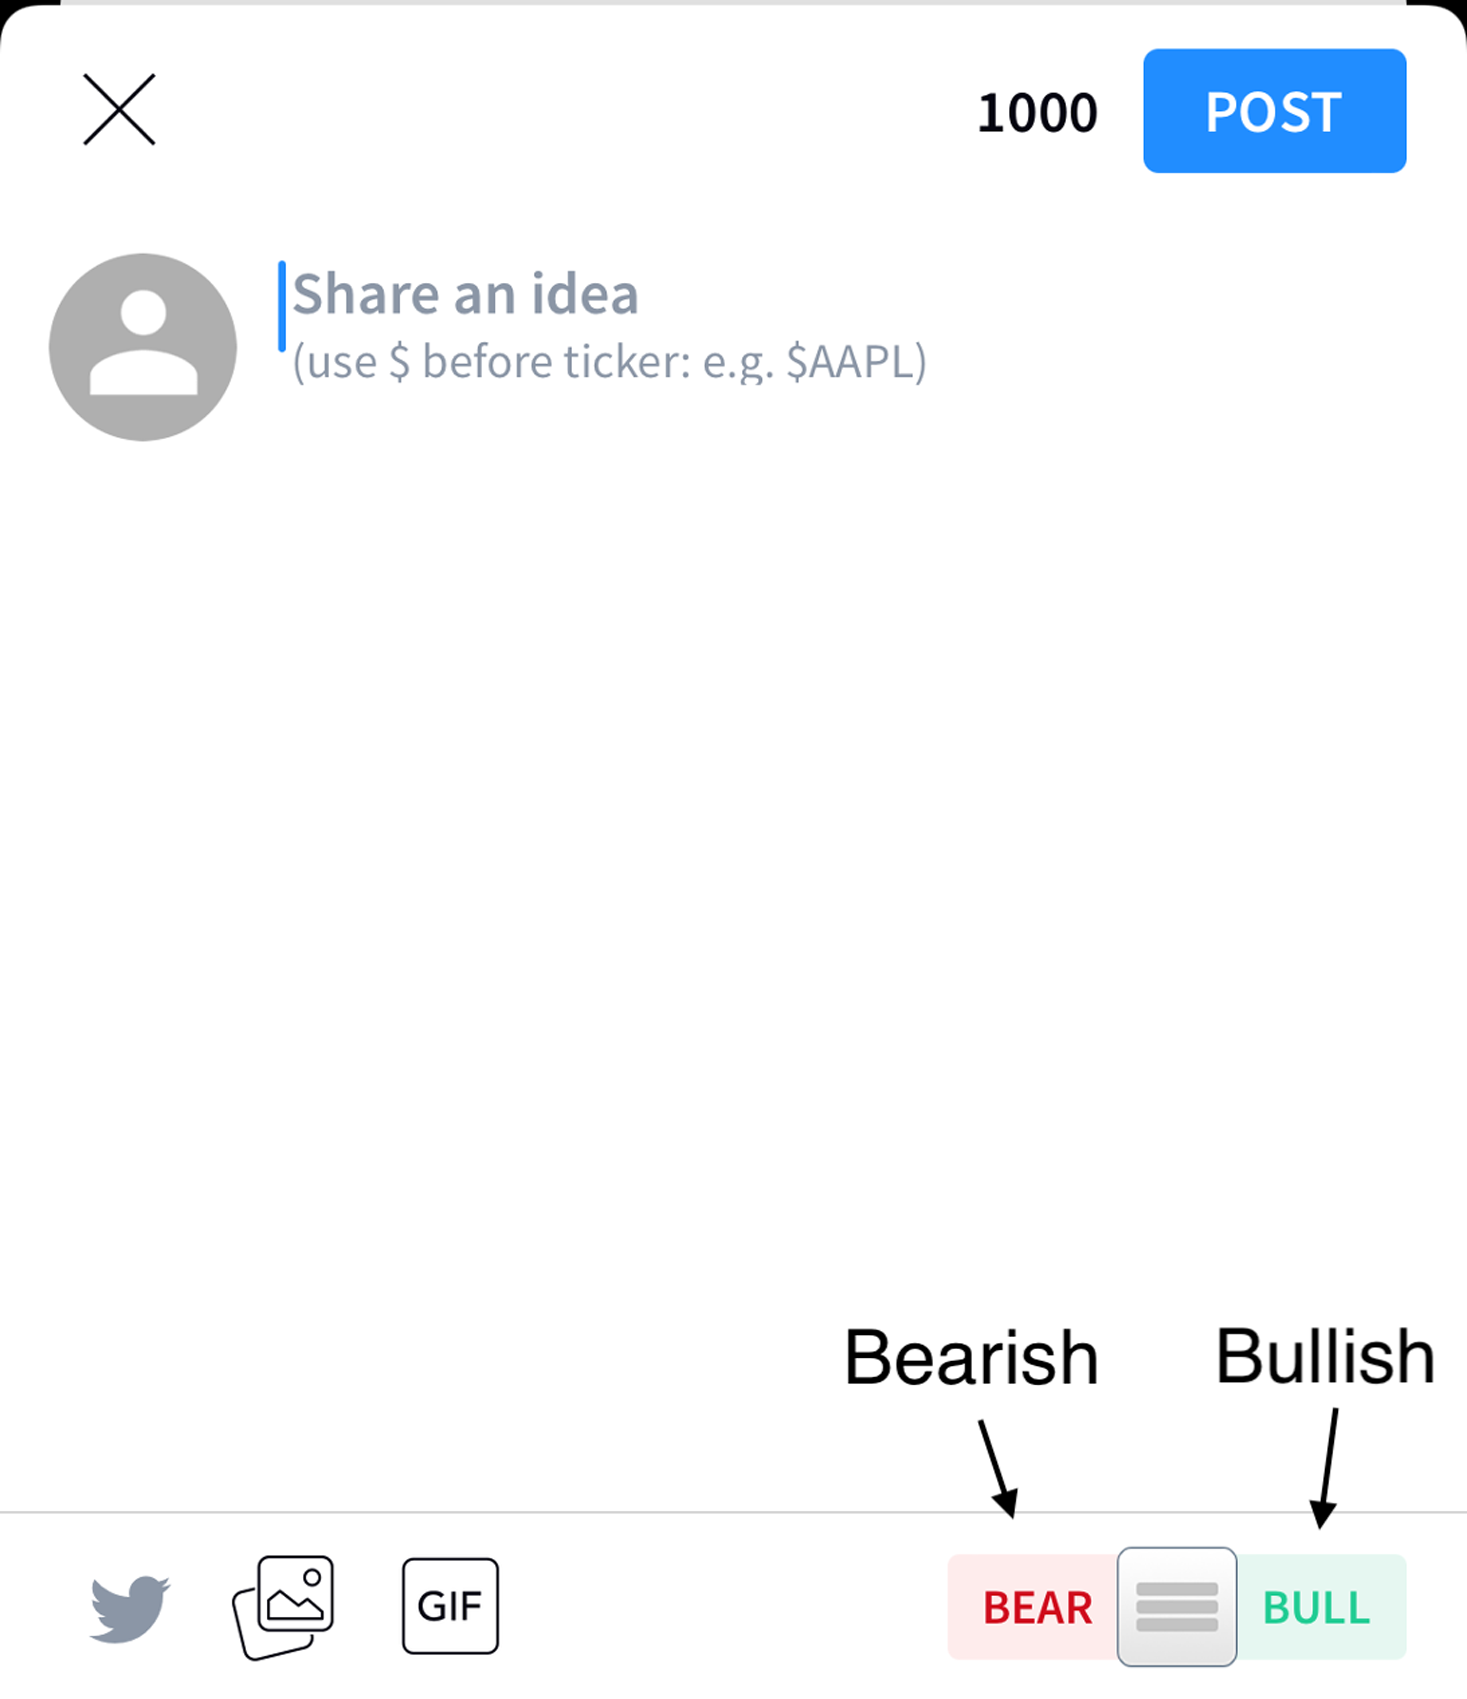
\includegraphics[width=0.6\linewidth]{gfx/m4l3_liu_fig1_stocktwits_ui.png}
\par\smallskip{\small \textbf{Hình 1:} Giao diện người dùng cho việc đăng bình luận và cảm xúc về các cổ phiếu cụ thể.}
\end{figure}

Trên Stocktwits, người dùng có tùy chọn gán nhãn bình luận của họ là tăng giá hoặc giảm giá, hoặc không gán nhãn. Điều này khiến việc dự đoán biến động cổ phiếu bằng cách phân tích cảm xúc trên Stocktwits trở nên khó khăn. Có nhiều cách tiếp cận để thu thập cảm xúc nhà đầu tư. Cách tiếp cận đơn giản nhất là (1) chỉ thu thập cảm xúc từ các bình luận đã được người dùng gán nhãn. Lý do là người dùng chủ động gán nhãn cảm xúc nên rủi ro phân loại sai giảm đi. Nhược điểm chính là dữ liệu cảm xúc có thể không đủ, dẫn đến chỉ số cảm xúc nhà đầu tư được tính toán không phản ánh đầy đủ cảm xúc thị trường. Do đó, hầu hết các nghiên cứu sử dụng một trong hai phương pháp sau: (2) sử dụng các bộ phân loại cảm xúc đa mục đích như VADER (Hutto \& Gilbert, 2014) hoặc Textblob (\url{https://textblob.readthedocs.io/en/dev/}) để phân tích tất cả bình luận (Koukaras, Nousi \& Tjortjis, 2022); (3) sử dụng tất cả các bình luận đã được người dùng gán nhãn trên Stocktwits để xây dựng một bộ phân loại cảm xúc và gán nhãn bình luận nhằm tăng lượng dữ liệu cảm xúc (Gupta \& Chen, 2020). Tuy nhiên, kết quả phân loại cảm xúc sẽ không hoàn toàn chính xác nếu dùng một mô hình phân loại cảm xúc để gán nhãn bình luận. Do đó, cần xem xét liệu có nên sử dụng một bộ phân loại cảm xúc trong việc dự đoán biến động giá cổ phiếu tương lai hay không.

Do thực tế là Stocktwits chỉ cho phép người dùng cung cấp nhãn cảm xúc tăng giá và giảm giá, điều này có thể dẫn đến việc tính toán không chính xác chỉ số cảm xúc cho các mô hình phân tích cảm xúc hai lớp. Điều này sẽ ảnh hưởng tiêu cực đến độ chính xác của dự đoán cổ phiếu. Để cải thiện độ chính xác của chỉ số cảm xúc cho dự đoán biến động giá cổ phiếu, chúng tôi đề xuất một cách tiếp cận mới lạ: sử dụng FinBERT (Araci, 2019), một mô hình phân tích cảm xúc tiên tiến nhất (state-of-the-art) trong lĩnh vực tài chính, để phân loại bình luận trên Stocktwits thành tích cực, tiêu cực, hoặc trung lập. Cách này có thể giảm đáng kể nhiễu, nhờ đó khắc phục một số hạn chế của việc sử dụng bộ phân loại cảm xúc hai lớp trên bình luận Stocktwits. Trong khi FinBERT thường được sử dụng để phân tích bài viết, tin tức và báo cáo tài chính, các nguồn dữ liệu này bị hạn chế và khó cung cấp dữ liệu thời gian thực với khối lượng lớn như mạng xã hội, điều thiết yếu để đạt được độ chính xác dự đoán lý tưởng. Do đó, chúng tôi áp dụng FinBERT để phân loại bình luận trên Stocktwits nhằm nâng cao mức độ hiểu biết vĩ mô của nó, nắm bắt cảm xúc tổng thể của một số lượng lớn nhà đầu tư và quan điểm của họ về các cổ phiếu cụ thể trên mạng xã hội.

Như đã đề cập, bộ phân loại cảm xúc được sử dụng trong nghiên cứu này là FinBERT. Sau khi phân loại cảm xúc, mục tiêu của chúng tôi là dự đoán biến động giá cổ phiếu tương lai. Trong các nghiên cứu trước đây, máy vector hỗ trợ (support vector machines, SVM) (Cortes \& Vapnik, 1995) đã được sử dụng để dự đoán giá cổ phiếu với kết quả xuất sắc (Tripathy, 2019). Hơn nữa, để nâng cao độ chính xác của dự đoán biến động giá cổ phiếu, chúng tôi đề xuất một mô hình mới lạ kết hợp kỹ thuật bagging (Breiman, 1996) với máy vector hỗ trợ. Ít nghiên cứu trong quá khứ đã đề cập đến việc kết hợp hai kỹ thuật này. Trong nghiên cứu này, chúng tôi so sánh hiệu suất của chúng thông qua năm thực nghiệm.

Ngoài ra, hầu hết các nghiên cứu hiện có dự đoán biến động giá giữa giá đóng cửa và giá mở cửa. Tuy nhiên, điều này không mang lại sự linh hoạt cho nhà đầu tư cần đưa ra quyết định giao dịch tức thì hoặc trong cùng ngày. Do đó, chúng tôi thu thập giá cổ phiếu trong phiên (intraday) để dự đoán biến động giá so với giá mở cửa.

Dựa trên những điều trên, các đóng góp chính của nghiên cứu này như sau:
\begin{enumerate}
  \item Chúng tôi thực hiện dự đoán biến động giá cổ phiếu dựa trên cảm xúc sử dụng FinBERT trên một mạng xã hội, Stocktwits, để nâng cao mức độ cảm xúc vĩ mô và cải thiện độ chính xác.
  \item Chúng tôi sử dụng nhiều kỹ thuật khác nhau để thu thập dữ liệu cảm xúc và so sánh hiệu suất của từng kỹ thuật trong việc dự đoán biến động giá cổ phiếu.
  \item Chúng tôi sử dụng máy vector hỗ trợ tập hợp (ensemble support vector machine) để nâng cao độ chính xác của dự đoán biến động giá cổ phiếu.
  \item Chúng tôi thay đổi thời điểm cắt (cut-off time) của dự đoán từ thời điểm đóng cửa sang thời điểm trong phiên (ví dụ: 12:00 giờ miền Đông Hoa Kỳ, EST) để tăng tính linh hoạt trong giao dịch.
\end{enumerate}

Cấu trúc của bài báo này như sau: Mục tiếp theo trình bày tổng quan ngắn gọn về phân tích cảm xúc và mô hình FinBERT, cũng như tổng quan các nghiên cứu gần đây về dự đoán biến động giá cổ phiếu dựa trên cảm xúc. Mục ``Phương pháp luận'' trình bày phương pháp được đề xuất cho dự đoán cổ phiếu, bao gồm thu thập và tiền xử lý dữ liệu, tính toán chỉ số cảm xúc, và máy vector hỗ trợ tập hợp được đề xuất. Mục ``Thiết lập thực nghiệm'' cung cấp tổng quan về chuẩn bị dữ liệu, trích xuất đặc trưng, xây dựng mô hình, và các chỉ số đánh giá. Mục ``Kết quả'' cung cấp chi tiết về từng thực nghiệm và kết quả tương ứng. Mục ``Thảo luận'' so sánh các phát hiện với các nghiên cứu trước đây. Cuối cùng, mục ``Kết luận'' tóm tắt các phát hiện nghiên cứu và vạch ra các định hướng nghiên cứu tương lai.

\section{Công trình liên quan}

Trong mục này, chúng tôi mô tả bối cảnh và các công trình liên quan gần đây trong dự đoán biến động giá cổ phiếu dựa trên cảm xúc. Điều này bao gồm các kỹ thuật phân tích cảm xúc, việc sử dụng máy vector hỗ trợ trong dự đoán giá cổ phiếu, các nghiên cứu liên quan gần đây, và mô hình FinBERT.

\subsection*{Các kỹ thuật phân tích cảm xúc}

Phân tích cảm xúc (sentiment analysis) là một lĩnh vực con của xử lý ngôn ngữ tự nhiên (natural language processing, NLP) có thể suy luận cảm xúc hoặc quan điểm của một cụm từ hoặc văn bản và phân loại nó là tích cực, tiêu cực, trung lập, v.v. (Sidogi, Mbuvha \& Marwala, 2021). Một trong những nguồn thu thập bình luận từ mọi người là mạng xã hội, và trong những năm gần đây, đã có nhiều nghiên cứu sử dụng những hiểu biết sâu sắc từ bình luận mạng xã hội để giải quyết nhiều vấn đề khác nhau. Shamoi và cộng sự (2022) đã sử dụng các bài đăng trên Twitter để tìm hiểu nhận thức của công chúng về chế độ ăn dựa trên thực vật và áp dụng các kỹ thuật phân tích cảm xúc để xác định liệu cảm xúc trong văn bản là tích cực hay tiêu cực. Những phát hiện này có thể giúp các chuyên gia y tế xây dựng các kế hoạch sức khỏe phù hợp và khuyến khích nhiều người hơn duy trì chế độ ăn dựa trên thực vật lành mạnh. Ko \& Chang (2021) đã thực hiện phân tích cảm xúc trên các bài đăng từ nền tảng PPT và sử dụng mô hình bộ nhớ ngắn hạn dài (long short-term memory, LSTM) để dự đoán giá cổ phiếu. Tuy nhiên, do bản chất phổ biến rộng rãi của mạng xã hội, có khả năng xảy ra các cuộc tấn công cá nhân hoặc phân biệt đối xử dựa trên chủng tộc và giới tính trên mạng xã hội. Raman và cộng sự (2022) giải thích rằng mặc dù nhiều công ty đã triển khai các thuật toán khác nhau trên nền tảng của họ, vẫn còn khó khăn trong việc phát hiện thường xuyên các bình luận như vậy, và chúng vẫn tiếp tục xuất hiện trên các nền tảng, gây ra tác động tiêu cực đến các nhóm đối tượng bị nhắm đến. Do đó, nghiên cứu đã so sánh các thuật toán phát hiện thù ghét và tấn công khác nhau để phát hiện lời nói mang cảm xúc thù ghét. Vì vậy, phân tích cảm xúc được ứng dụng rộng rãi và mang lại giá trị thương mại đáng kể.

\subsection*{Dự đoán biến động giá cổ phiếu dựa trên cảm xúc sử dụng máy vector hỗ trợ}

Máy vector hỗ trợ (SVM) là một kỹ thuật học có giám sát được giới thiệu bởi Cortes \& Vapnik (1995), có thể được sử dụng để giải quyết các vấn đề liên quan đến cả hồi quy và phân loại. SVM có thể đạt hiệu suất cao trong các nhiệm vụ phân loại, với điều kiện được trang bị hàm nhân (kernel). Khi dữ liệu trong không gian ban đầu không thể được phân tách bằng một bộ phân loại tuyến tính, hàm nhân được dùng để thực hiện phép chiếu phi tuyến, nhằm phân tách dữ liệu trong một không gian có số chiều cao hơn. Do thực tế thị trường chứng khoán là một ví dụ điển hình của hệ thống phi tuyến, động (non-linear, dynamic), SVM thường được sử dụng để dự đoán giá cổ phiếu. Mặc dù SVM hoạt động tốt trong việc giải quyết các bài toán phân loại, nó vẫn có một số nhược điểm. Theo Auria \& Moro (2008), một nhược điểm của SVM là thiếu tính minh bạch của kết quả, khiến việc lấy điểm và xác suất phân loại trở nên khó khăn. Hạn chế này có thể cản trở khả năng đưa ra quyết định linh hoạt, đặc biệt khi mua hoặc bán dựa trên xác suất của kết quả phân loại.

Theo phát hiện của Hu, Zhu \& Tse (2013), SVM có khả năng tổng quát hóa tốt cũng như khả năng chống chịu mạnh đối với vấn đề quá khớp (overfitting). Ngược lại, việc huấn luyện một mô hình SVM tương tự như giải một bài toán quy hoạch bậc hai bị ràng buộc tuyến tính, và phân loại SVM luôn tạo ra một nghiệm tối ưu toàn cục duy nhất. Điều này trái ngược với việc huấn luyện một mạng nơ-ron, vốn đòi hỏi tối ưu hóa phi tuyến và có nguy cơ rơi vào nghiệm cực tiểu cục bộ. Ngoài ra, nghiên cứu đó dự đoán giá cổ phiếu bằng cách kết hợp báo cáo thường niên và các yếu tố kinh tế vĩ mô. Các phát hiện cuối cùng chứng minh rằng SVM là một kỹ thuật dự đoán hữu ích để sử dụng trong dự báo cổ phiếu.

Ren, Wu \& Liu (2019) cho rằng các đặc trưng cảm xúc có thể chứa thông tin giá trị về giá trị cơ bản của tài sản và có thể được coi là một trong những chỉ báo dẫn đầu của thị trường chứng khoán. Họ cũng đề cập rằng SVM có thể giải quyết các vấn đề phi tuyến bằng cách chuyển đổi chúng thành quy hoạch bậc hai và có một nghiệm tối ưu toàn cục duy nhất, khiến nó trở thành công cụ hữu ích để dự đoán biến động giá của thị trường chứng khoán. Các nhà nghiên cứu đã triển khai kiểm định chéo năm lần (fivefold cross validation) bằng SVM, nhưng phát hiện rằng làm như vậy gây ra thiên lệch nhìn trước (look-ahead bias). Để loại bỏ thiên lệch này, họ đã tích hợp SVM với phương pháp cửa sổ trượt (rolling window) thực tế. Để tránh quá khớp trong nghiên cứu của chúng tôi, phương pháp cửa sổ trượt sẽ được sử dụng để kiểm chứng hiệu quả của nó.

\subsection*{Sử dụng bình luận Stocktwits để dự đoán biến động giá cổ phiếu dựa trên cảm xúc}

Trong một nghiên cứu được thực hiện bởi Koukaras, Nousi \& Tjortjis (2022), các bình luận được thu thập từ người dùng trên Twitter và Stocktwits, và biến động giá cổ phiếu được dự đoán thông qua phân tích cảm xúc và học máy. Nghiên cứu sử dụng VADER làm bộ phân tích cảm xúc và dự đoán xu hướng giá cổ phiếu của Microsoft (MSFT). Nhiều mô hình học máy khác nhau đã được thử nghiệm để dự đoán biến động giá cổ phiếu, và kết quả cuối cùng cho thấy SVM vượt trội hơn các mô hình phân loại khác. Nghiên cứu này đã sử dụng phân tích cảm xúc trên mạng xã hội để dự báo cổ phiếu tại thị trường Mỹ, đạt được kết quả tốt và truyền cảm hứng cho các nhà nghiên cứu sử dụng SVM để giải quyết bài toán dự đoán biến động giá cổ phiếu dựa trên cảm xúc trong nghiên cứu của họ.

Gupta \& Chen (2020) đã thu thập dữ liệu bình luận từ Stocktwits trong khoảng thời gian từ ngày 1 tháng 1 năm 2019 đến ngày 30 tháng 9 năm 2019. Họ đã phát triển một số bộ phân tích cảm xúc cho các cổ phiếu khác nhau bằng các kỹ thuật như hồi quy logistic và TF-IDF. Sau đó, họ đã thử nghiệm với một số cổ phiếu Mỹ để dự đoán biến động giá cổ phiếu và phát hiện rằng việc bổ sung nhiều dữ liệu cảm xúc hơn giúp cải thiện độ chính xác của dự đoán biến động giá cổ phiếu.

Hơn nữa, trong những năm gần đây, nhiều nghiên cứu đã phát triển các mô hình phân tích cảm xúc hai lớp sử dụng bình luận trên Stocktwits. Điều này có ích cho nghiên cứu và so sánh của chúng tôi. Lee, Gao \& Tsai (2020) đã tinh chỉnh (fine-tune) BERT đã được huấn luyện trước trên một bộ dữ liệu cảm xúc đã gán nhãn và đạt độ chính xác trên 87.3\% trong việc nhận diện cảm xúc của nhà đầu tư. Bozanta và cộng sự (2021) đã tiến hành nhiều thực nghiệm và cuối cùng sử dụng RoBERTa (Liu và cộng sự, 2019) để đạt độ chính xác 83 đến 88\%. Cao và cộng sự (2022) đã tinh chỉnh mô hình roberta-base trên 3.2 triệu bình luận từ Stocktwits, với các nhãn tăng giá hoặc giảm giá do người dùng gán, và đạt được độ chính xác kiểm định 93.43\%. Do đó, nghiên cứu của chúng tôi sử dụng mô hình được đề xuất bởi Cao và cộng sự (2022) cho phân tích cảm xúc hai lớp để dự đoán biến động giá cổ phiếu và so sánh nó với phương pháp được đề xuất trong bài báo này.

\subsection*{FinBERT: phân tích cảm xúc tài chính với BERT}

FinBERT (Araci, 2019) là ứng dụng đầu tiên của BERT (Devlin và cộng sự, 2018) trong lĩnh vực tài chính, là một mô hình phân tích cảm xúc đã được huấn luyện trước chuyên biệt cho việc phân tích văn bản tài chính. FinBERT trước tiên huấn luyện trước (pre-train) mô hình ngôn ngữ BERT bằng một tập dữ liệu tài chính lớn, sau đó tinh chỉnh (fine-tune) nó trên một tập dữ liệu tài chính cụ thể (\url{https://huggingface.co/ProsusAI/finbert}). FinBERT đạt mức tiên tiến nhất (SOTA, state-of-the-art) trên bộ dữ liệu Financial Phrasebank. Bộ dữ liệu này gồm 4,840 câu tin tức tài chính bằng tiếng Anh được phân loại theo cảm xúc (Malo và cộng sự, 2013). Độ chính xác của mô hình cao hơn 15\% so với mô hình tiên tiến nhất hiện tại. Mô hình có thể tạo ra ba loại phân loại cảm xúc, bao gồm tích cực, tiêu cực, và trung lập, cho phép chúng ta phát hiện cảm xúc trung lập và tính toán chỉ số cảm xúc chính xác hơn, từ đó nâng cao độ chính xác của dự đoán biến động giá cổ phiếu. FinBERT cho phân tích cảm xúc thường được sử dụng để phân tích tin tức và bài viết tài chính. FinBERT thực hiện phân loại cảm xúc bằng cách thêm một lớp kết nối đầy đủ (dense layer) sau trạng thái ẩn cuối cùng của token [CLS], đây là phương pháp được khuyến nghị để sử dụng BERT cho bất kỳ nhiệm vụ phân loại nào. Mạng phân loại sau đó được huấn luyện trên một tập dữ liệu cảm xúc đã gán nhãn. Quy trình được tóm tắt trong Hình 2.

\begin{figure}[H]
\centering
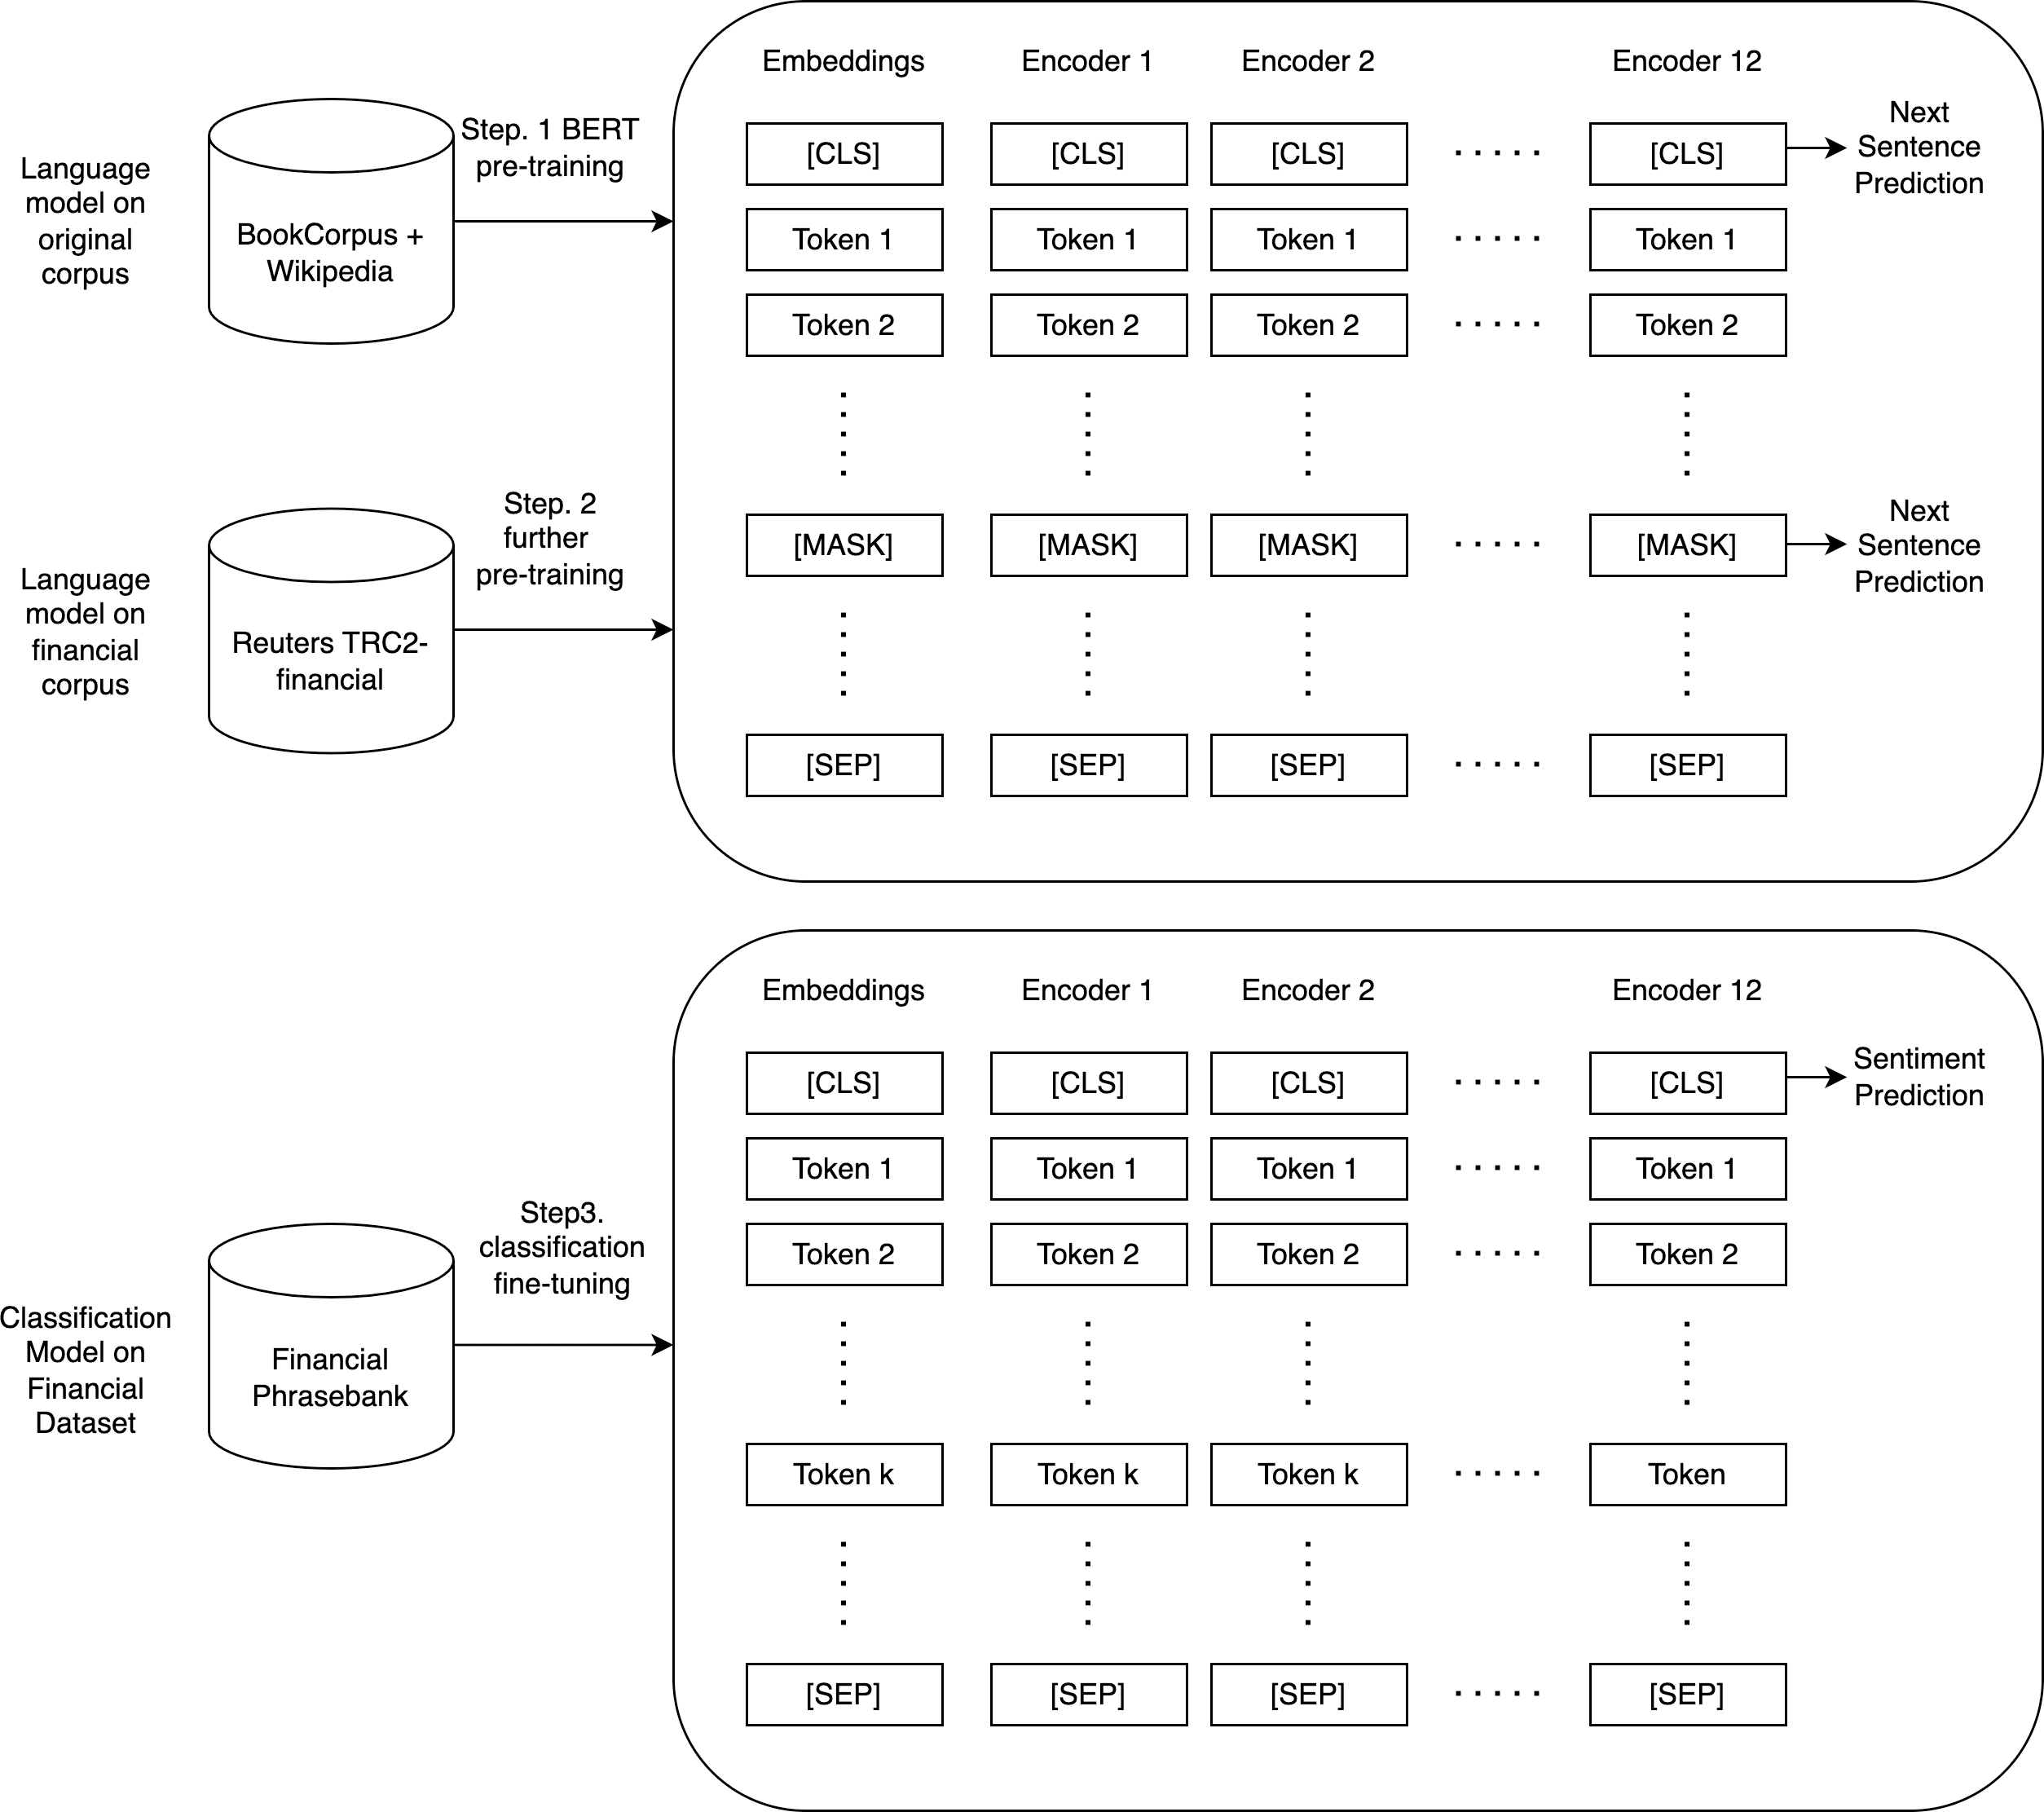
\includegraphics[width=0.85\linewidth]{gfx/m4l3_liu_fig2_pretraining_overview.png}
\par\smallskip{\small \textbf{Hình 2:} Tổng quan về huấn luyện trước, huấn luyện trước bổ sung, phân loại, và tinh chỉnh của FinBERT.}
\end{figure}

Fazlija \& Harder (2022) đã sử dụng mô hình FinBERT để phân loại tin tức, dự báo xu hướng giá cổ phiếu bằng bộ phân loại rừng ngẫu nhiên (random forest), và đo lường hiệu suất đầu tư của các mô hình. Hiệu suất của phương pháp được đề xuất trong nghiên cứu vượt trội hơn chỉ số S\&P 500. Tuy nhiên, mặc dù bài báo này sử dụng kiểm định chéo K-lần (K-fold cross-validation) để tìm tham số mô hình tốt nhất, chia tập dữ liệu huấn luyện và kiểm định thành nhiều bản sao, và huấn luyện nhiều mô hình để kiểm định, các tác giả không đề cập đến việc sử dụng phương pháp cửa sổ trượt trong nghiên cứu của họ. Do đó, trong nghiên cứu của chúng tôi, chúng tôi dự định áp dụng FinBERT để phân tích các bình luận trên mạng xã hội, cho phép chúng tôi thu thập nhiều ý kiến hơn về tài sản mục tiêu. Sau đó, bằng cách dự đoán sử dụng phương pháp cửa sổ trượt, chúng tôi không chỉ có thể tránh vấn đề thiên lệch nhìn trước, mà còn cập nhật dữ liệu huấn luyện theo thời gian, điều này có thể dẫn đến các dự đoán chính xác hơn.

Trong nghiên cứu này, chúng tôi đề xuất sử dụng FinBERT để thực hiện phân tích cảm xúc trên bình luận của nhà đầu tư trên Stocktwits nhằm dự đoán biến động giá cổ phiếu. Ít nghiên cứu đã sử dụng FinBERT để phân tích cảm xúc trên mạng xã hội. Tuy nhiên, chúng tôi tin rằng việc áp dụng nó cụ thể để phân tích bình luận Stocktwits, thay vì sử dụng mô hình phân tích cảm xúc hai lớp, sẽ cải thiện chỉ số cảm xúc ở mức vĩ mô và nâng cao độ chính xác của dự đoán biến động giá cổ phiếu.

\section{Phương pháp luận}

Trong mục này, chúng tôi thảo luận về các nguồn dữ liệu khác nhau có thể được sử dụng để phân tích cổ phiếu, chẳng hạn như dữ liệu lịch sử, bình luận, và dữ liệu cảm xúc. Chúng tôi cũng trình bày các bước tiền xử lý cần thiết để phân tích bình luận, bao gồm cách tính toán chỉ số cảm xúc. Cuối cùng, chúng tôi giới thiệu một mô hình dự đoán biến động giá cổ phiếu sử dụng các kỹ thuật tập hợp (ensemble) và máy vector hỗ trợ.

\subsection*{Thu thập dữ liệu}

Trên Stocktwits, người dùng có thể chia sẻ một tin nhắn và gán nhãn nó là ``tăng giá'' (bullish) hoặc ``giảm giá'' (bearish), hoặc họ có thể bỏ qua các cảm xúc này. Có ba cột dữ liệu: tin nhắn, ngày/giờ, và cảm xúc (tùy chọn). Các tin nhắn (tweets) trên Stocktwits được thể hiện trong Hình 3.

\begin{figure}[H]
\centering

\includegraphics[width=0.6\linewidth]{gfx/m4l3_liu_fig3_tweets_stocktwits.png}
\par\smallskip{\small \textbf{Hình 3:} Các tin nhắn được người dùng đăng trên Stocktwits. Người dùng có thể điền văn bản và gán nhãn cảm xúc theo quan điểm của họ về tương lai (tùy chọn). Như có thể thấy trong hình, một số tin nhắn có cảm xúc tăng giá hoặc giảm giá, trong khi những tin nhắn khác không được gán nhãn.}
\end{figure}

Việc truy cập \url{https://api.Stocktwits.com/} cho phép chúng tôi xem xét các bình luận của nhà đầu tư ở định dạng JSON về một cổ phiếu nhất định từ Stocktwits. Để lấy dữ liệu từ Stocktwits, chúng tôi đã phát triển một ứng dụng Node.js tự động tải xuống và lưu các tệp CSV chứa tất cả bình luận về một cổ phiếu cụ thể trong một khoảng thời gian nhất định. Sau đó, chúng tôi đưa dữ liệu vào môi trường Python để thực hiện phân tích sâu hơn.

Dữ liệu cổ phiếu lịch sử được thu thập từ cnYES (\url{https://www.cnyes.com/}), và các cột dữ liệu bao gồm giá mở cửa, giá đóng cửa, giá cao nhất, giá thấp nhất của cổ phiếu, VWAP (giá bình quân gia quyền theo khối lượng), khối lượng, giá trị giao dịch, mức thay đổi, và phần trăm thay đổi, như được thể hiện trong Bảng 1.

\begin{figure}[H]
\centering
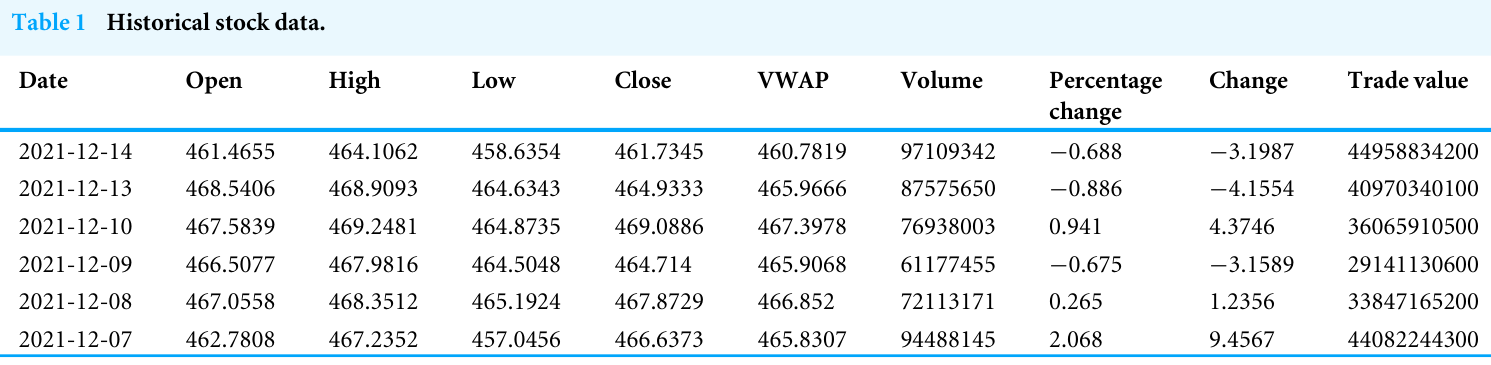
\includegraphics[width=0.95\linewidth]{gfx/m4l3_liu_table1_historical_stock_data.png}
\par\smallskip{\small \textbf{Bảng 1:} Dữ liệu cổ phiếu lịch sử.}
\end{figure}

Chúng tôi đã sử dụng AlphaVantage API (\url{https://www.alphavantage.co/}) để lấy dữ liệu giá cổ phiếu lịch sử theo thời gian thực. Điều này cho phép chúng tôi nắm được thông tin chi tiết về giá cổ phiếu theo từng phút, giúp chúng tôi đưa ra các dự báo linh hoạt hơn. Tuy nhiên, dữ liệu bị giới hạn trong hai năm gần nhất. Bảng 2 cho thấy dữ liệu giá cổ phiếu lịch sử với bước thời gian 15 phút.

\begin{figure}[H]
\centering
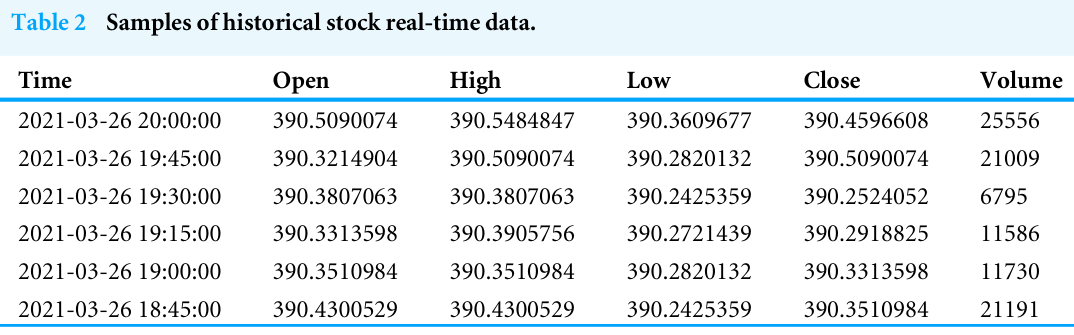
\includegraphics[width=0.85\linewidth]{gfx/m4l3_liu_table2_realtime_data_samples.png}
\par\smallskip{\small \textbf{Bảng 2:} Mẫu dữ liệu giá cổ phiếu lịch sử thời gian thực.}
\end{figure}

\subsection*{Tiền xử lý dữ liệu cảm xúc}

Chúng tôi tham khảo Cao và cộng sự (2022). Trước khi thực hiện phân tích cảm xúc, các bước tiền xử lý văn bản sau đây cần được thực hiện:
\begin{enumerate}
  \item Loại bỏ tất cả các liên kết web khỏi văn bản, bao gồm cả những liên kết bắt đầu bằng ``http://'', ``https://'', hoặc ``www.''.
  \item Thay thế ký tự HTML cho dấu nháy đơn bằng dấu nháy đơn tiêu chuẩn.
  \item Nhận diện và thay thế các hashtag (\#) và cashtag (\$) trong văn bản. Tìm tất cả các từ bắt đầu bằng ``\#'' hoặc ``\$'', chẳng hạn như \$AAPL, và thay thế chúng bằng các thuật ngữ như ``cashtag\_AAPL''. Sự thay đổi này được thực hiện nhằm bảo toàn thông tin ký hiệu gốc đồng thời làm cho nó phù hợp hơn cho việc xử lý văn bản.
  \item Thay thế tên người dùng Twitter bằng một thuật ngữ bắt đầu bằng ``mention\_'', theo sau là tên người dùng. Sửa đổi này cũng nhằm mục đích bảo toàn thông tin gốc trong khi làm cho nó phù hợp hơn cho việc xử lý văn bản.
  \item Chuyển đổi tất cả biểu tượng cảm xúc (emoji) thành mô tả văn bản tương ứng để duy trì thông tin cảm xúc hoặc ngữ nghĩa mà chúng truyền tải, nhưng ở một định dạng dễ hiểu hơn đối với mô hình.
\end{enumerate}

\subsection*{Dự đoán biến động giá cổ phiếu}

Kiến trúc được mô tả trong Hình 4 được sử dụng để dự đoán biến động giá cổ phiếu. Chúng tôi thu thập dữ liệu cần thiết, được chia thành hai phần: phần đầu tiên bao gồm các bình luận về các cổ phiếu cụ thể trên Stocktwits, một số trong đó không được gán nhãn tăng giá hoặc giảm giá, trong khi phần thứ hai bao gồm dữ liệu lịch sử về giá cổ phiếu. Chúng tôi có thể chọn sử dụng mô hình phân tích cảm xúc hai lớp để gán nhãn các bình luận chưa được gán nhãn hoặc sử dụng mô hình phân tích cảm xúc ba lớp như FinBERT hoặc VADER để gán nhãn tất cả bình luận. Cuối cùng, chúng tôi áp dụng công thức chỉ số cảm xúc để tính chỉ số thực thể (entity index) của các bình luận từ nhiều giai đoạn khác nhau. Để dự đoán biến động giá cổ phiếu, chúng tôi kết hợp các chỉ số cảm xúc với dữ liệu cổ phiếu lịch sử làm đặc trưng và đưa chúng vào một mô hình dự đoán được thiết kế cho biến động giá cổ phiếu. Chúng tôi đã sử dụng phương pháp cửa sổ trượt để dự đoán và phân tích độ chính xác của các dự đoán biến động cổ phiếu.

\begin{figure}[H]
\centering
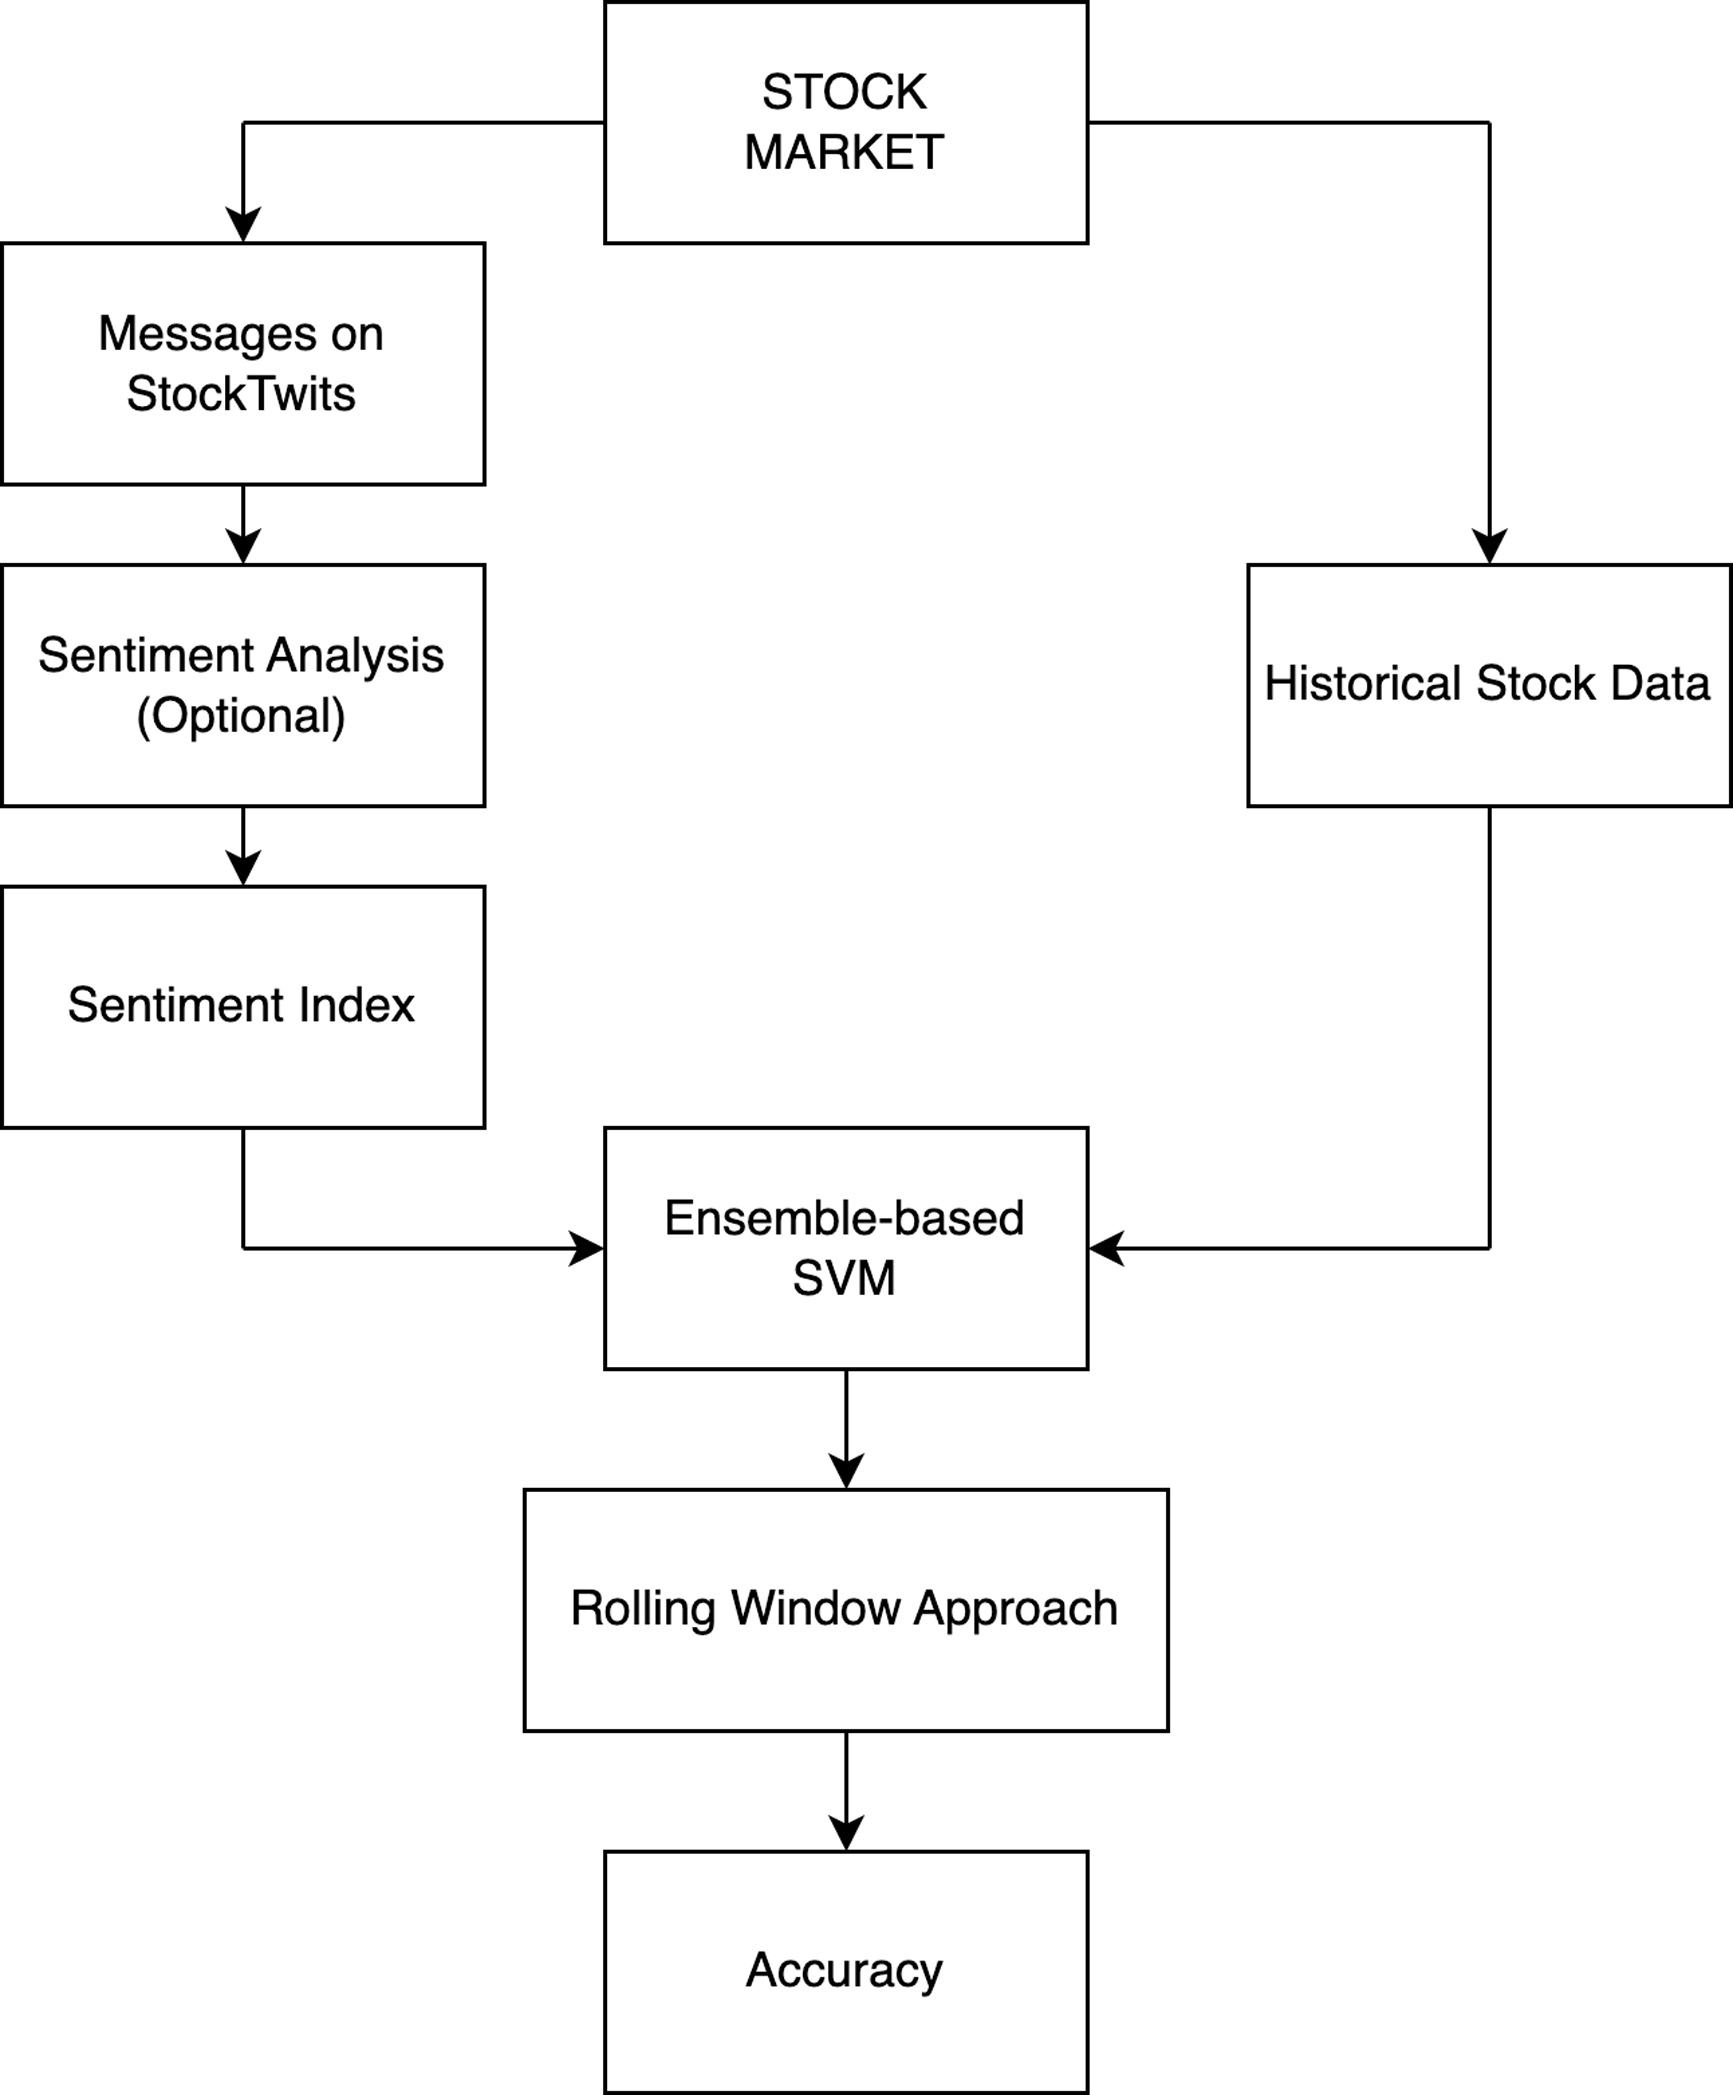
\includegraphics[width=0.55\linewidth]{gfx/m4l3_liu_fig4_prediction_architecture.png}
\par\smallskip{\small \textbf{Hình 4:} Tổng quan kiến trúc dự đoán biến động thị trường chứng khoán.}
\end{figure}

\subsection*{Tính toán chỉ số cảm xúc}

Cách tính chỉ số cảm xúc hai lớp được sử dụng trong bài báo này tham khảo phương pháp của Antweiler \& Frank (2004).

$$
S_t = \ln\left[\frac{1+M_t^{pos}}{1+M_t^{neg}}\right]
$$

Chỉ số này cho phép chúng ta tính toán cảm xúc cho một giai đoạn, trong đó $M_t^{pos}$, $M_t^{neg}$ là số lượng tin nhắn tích cực và tiêu cực trong giai đoạn đó. Nếu chỉ số cảm xúc dương, cảm xúc thị trường là lạc quan. Nếu chỉ số cảm xúc âm, cảm xúc thị trường là bi quan. Nếu chỉ số cảm xúc bằng không, cảm xúc thị trường là trung lập. Chỉ số này giúp chúng tôi xác định cảm xúc nhà đầu tư trong một khoảng thời gian nhất định và cũng điều chỉnh cho các tín hiệu quá lạc quan hoặc quá bi quan trong quá trình tính toán.

Đối với các mô hình phân tích cảm xúc ba lớp (bao gồm cảm xúc tích cực, tiêu cực, và trung lập), tham khảo phương trình được sử dụng để tính chỉ số cảm xúc trong Hiew và cộng sự (2019).

$$
S_t = \frac{M_t^{pos} - M_t^{neg}}{M_t^{pos} + M_t^{neu} + M_t^{neg}}
$$

trong đó $M_t^{pos}$, $M_t^{neg}$, $M_t^{neu}$ là số lượng tin nhắn tích cực, tiêu cực và trung lập trong giai đoạn đó.

\subsection*{Máy vector hỗ trợ}

Máy vector hỗ trợ (SVM) là một thuật toán học máy có giám sát được phát triển bởi Cortes \& Vapnik (1995), có thể được sử dụng để giải quyết các bài toán phân loại và hồi quy. Khái niệm này khá đơn giản: tìm một ranh giới quyết định (decision boundary) tối đa hóa biên (margin) giữa hai lớp, như được thể hiện trong Hình 5.

\begin{figure}[H]
\centering
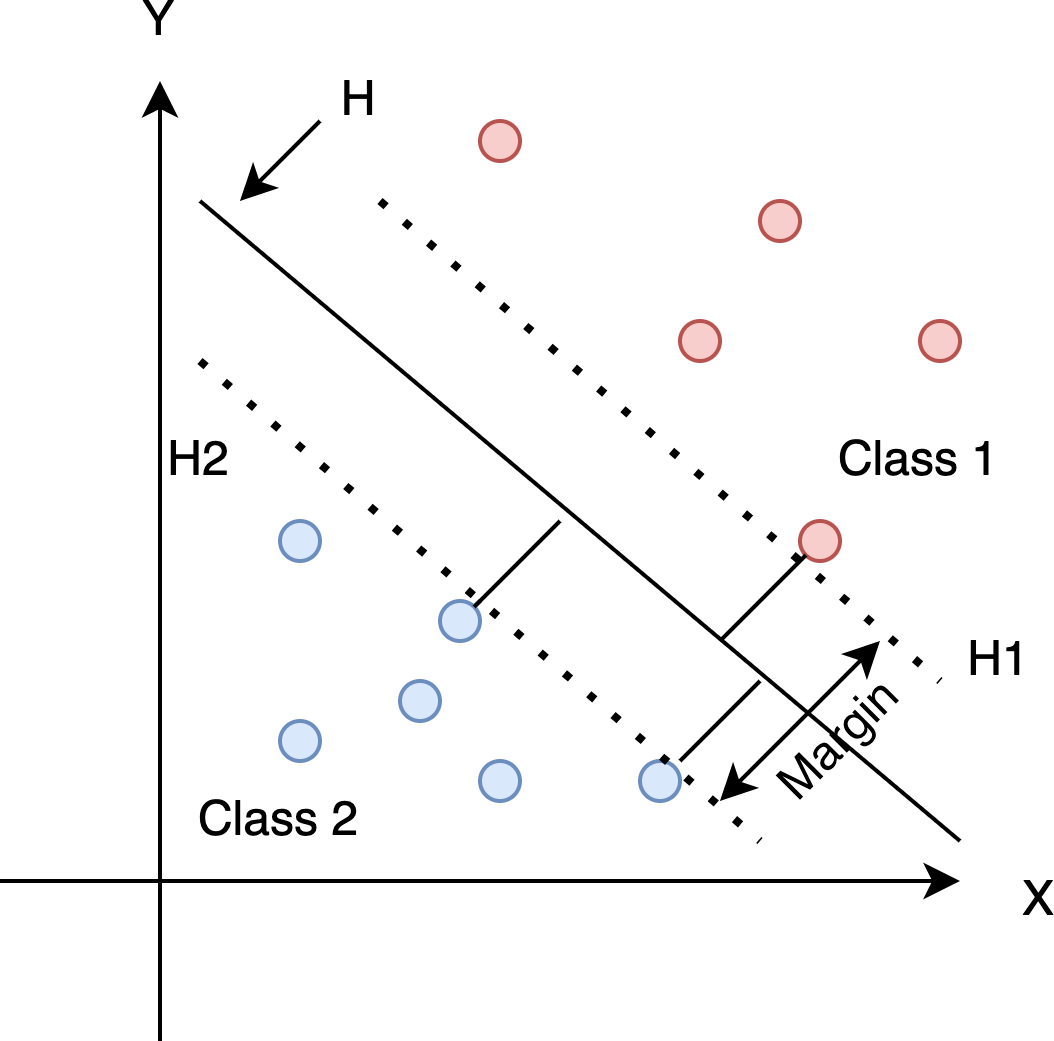
\includegraphics[width=0.6\linewidth]{gfx/m4l3_liu_fig5_svm_hyperplane.png}
\par\smallskip{\small \textbf{Hình 5:} Tìm siêu phẳng (hyperplane) tối ưu phân tách tập dữ liệu thành hai loại.}
\end{figure}

Khoảng cách từ điểm $(x, y)$ đến đường thẳng $Ax+By+C=0$ được cho bởi

$$
\frac{Ax+By+C}{\sqrt{A^2+B^2}}
$$

Mở rộng nó sang không gian $n$ chiều, chúng ta biểu diễn nó là $w^T x + b = 0$, và khoảng cách là

$$
\frac{(w^T x + b)}{\lVert w \rVert}
$$

trong đó $w$ biểu thị trọng số của mỗi đặc trưng, $b$ biểu thị hệ số chặn (intercept).

Nếu chúng ta bỏ qua vấn đề dữ liệu trộn lẫn, tức là nếu tất cả dữ liệu có thể được phân loại hoàn hảo, chúng ta gọi đây là SVM biên cứng (hard-margin SVM) và phân chia hai lớp theo phương trình dưới đây.

$$
\begin{cases}
w^T x^{(i)} + b \geq 1, & \forall y^{(i)} = 1 \\
w^T x^{(i)} + b \leq -1, & \forall y^{(i)} = -1
\end{cases}
$$

Và đơn giản hóa công thức như sau

$$
y^{(i)}\left(w^T x^{(i)} + b\right) \geq 1, \quad \forall i = 1, \dots, n
$$

Nghiệm của SVM là một bài toán tối ưu hóa đơn giản. Trong một số điều kiện, khoảng cách biên giữa hai lớp càng lớn thì càng tốt. Công thức như sau

$$
\min \frac{1}{2} \lVert w \rVert^2
$$

$$
\text{s.t.} \quad y_i\left(w^T x_i + b\right) \geq 0, \quad \forall i = 1, \dots, n
$$

Tuy nhiên, hiếm khi dữ liệu thực tế bao gồm các ví dụ có thể được xác định chính xác. Do đó, chúng ta cho phép một số điểm nhất định vượt qua ranh giới quyết định ban đầu và cho phép một số mẫu bất thường bị phân loại sai. Mặc dù điều này có thể dẫn đến việc phân loại sai, khả năng tổng quát hóa có thể tốt hơn trong các ứng dụng thực tế. Loại SVM này được gọi là SVM biên mềm (soft-margin SVM), sử dụng công thức sau

$$
\min_{w, \xi_i} \frac{1}{2} w^T w + C \sum_{i=1}^{n} \xi_i
$$

$$
\text{s.t.} \quad y_i\left(w^T x_i + b\right) \geq 1 - \xi_i, \; \xi_i \geq 0, \; \forall i = 1, \dots, n
$$

trong đó $\xi_i$ là một sai số huấn luyện có thể chấp nhận được, và $C$ xác định mức trọng số phạt cần được đưa ra.

Từ phương trình trên, chúng ta có thể thấy rằng nếu $C$ lớn hơn, mức dung sai đối với lỗi nhỏ hơn, và nếu $C$ tiến tới dương vô cực, nó sẽ trở thành SVM biên cứng. Ngược lại, nếu $C$ nhỏ hơn, mức dung sai đối với lỗi lớn hơn.

Để giải nghiệm tối ưu của bài toán gốc (primal problem), chúng ta có thể chuyển đổi nó thành bài toán đối ngẫu (dual problem), như được thể hiện trong phương trình sau

$$
\max_{\alpha} \sum_{i=1}^{n} \alpha_i - \frac{1}{2} \sum_{i=1}^{n} \sum_{j=1}^{n} \alpha_i \alpha_j y_i y_j K(x_i, x_j)
$$

$$
\text{s.t.} \quad \sum_{i=1}^{n} \alpha_i y_i = 0
$$

$$
0 \leq \alpha_i \leq C, \quad \forall i = 1, \dots, n
$$

trong đó $\boldsymbol{\alpha} = (\alpha_1, \dots, \alpha_n)^T$ là nhân tử Lagrange, và $K(x_i, x_j)$ biểu thị việc chúng ta sử dụng một hàm nhân (kernel) để định nghĩa lại tích trong (inner product) của $x_i$ và $x_j$. Có một số hàm nhân phổ biến được thể hiện trong Bảng 3.

\begin{figure}[H]
\centering
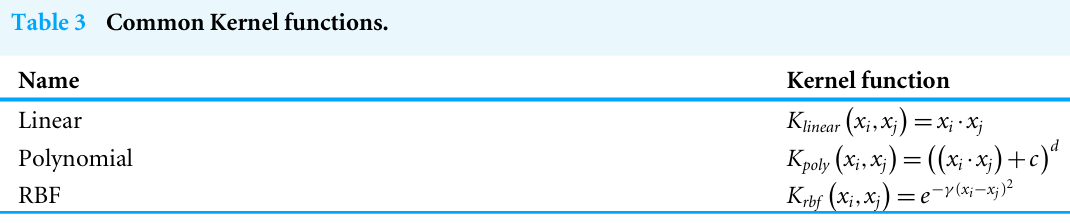
\includegraphics[width=0.9\linewidth]{gfx/m4l3_liu_table3_kernel_functions.png}
\par\smallskip{\small \textbf{Bảng 3:} Các hàm nhân (kernel function) phổ biến.}
\end{figure}

Cuối cùng, hàm quyết định $D(x) = \operatorname{sgn}(w^* \cdot x + b^*)$ được cho bởi

$$
D(x) = \operatorname{sgn}\left(\sum_{i=1}^{n} y_i \alpha_i * K(x_i, x_j) + b^*\right)
$$

$$
b^* = y_j - \sum_{i=1}^{n} y_i \alpha_i * K(x_i, x_j)
$$

\subsection*{Kỹ thuật dựa trên tập hợp (ensemble)}

Theo Mohareb và cộng sự (2016), kỹ thuật dựa trên tập hợp (ensemble-based) dựa trên việc phát triển nhiều bộ phân loại, với đầu ra dự đoán cuối cùng là sự tổng hợp của tất cả các kết quả phân loại trong tập hợp đó. Giả sử chúng ta sử dụng $n$ bộ phân loại $\varepsilon = \{C_1, \dots, C_n\}$ để dự đoán một mẫu, nếu kết quả của $C_1$ sai, nhưng kết quả của $C_2, \dots, C_n$ đúng, thì kết quả có thể được phân loại chính xác bằng cách bỏ phiếu đa số (majority voting).

Các bộ phân loại riêng lẻ phải có độ chính xác tốt để phương pháp này khả thi. Nếu có tổng cộng $T$ bộ phân loại cho một bài toán $c$ lớp, lựa chọn tập hợp sẽ đúng nếu ít nhất $[T/c+1]$ bộ phân loại chọn đúng lớp. Giả sử mỗi bộ phân loại của $\varepsilon$ có xác suất $p$ chọn đúng lớp. Xác suất tập hợp chọn đúng lớp tuân theo phân phối nhị thức, và xác suất chọn được $k > T/c+1$ bộ phân loại đúng trong số $T$ được tính như sau (Mohareb và cộng sự, 2016):

$$
p_\varepsilon = \sum_{k=(T/c)+1}^{T} \binom{T}{k} p^k (1-p)^{(T-k)}
$$

\subsection*{Tập hợp SVM với bagging}

Theo Kim và cộng sự (2002), trong bagging, nhiều SVM được huấn luyện riêng lẻ bằng phương pháp bootstrap và sau đó được tổng hợp bằng một kỹ thuật kết hợp phù hợp. Tập huấn luyện cần được chia thành $L$ tập con để xây dựng tập hợp SVM với $L$ máy SVM độc lập. Dựa trên bằng chứng thống kê, cần làm cho các tập huấn luyện đa dạng nhất có thể để đạt được cải thiện lớn hơn trong kết quả tổng hợp. Chúng tôi áp dụng phương pháp bootstrap để thực hiện điều này.

Phương pháp bootstrap được đề xuất bởi Efron (1979). Nói một cách đơn giản, mỗi mô hình được huấn luyện bằng cách chọn ngẫu nhiên $n$ mẫu dữ liệu từ tập huấn luyện, và mỗi mẫu được trả lại tập huấn luyện sau khi chọn, như được thể hiện trong Hình 6.

\begin{figure}[H]
\centering
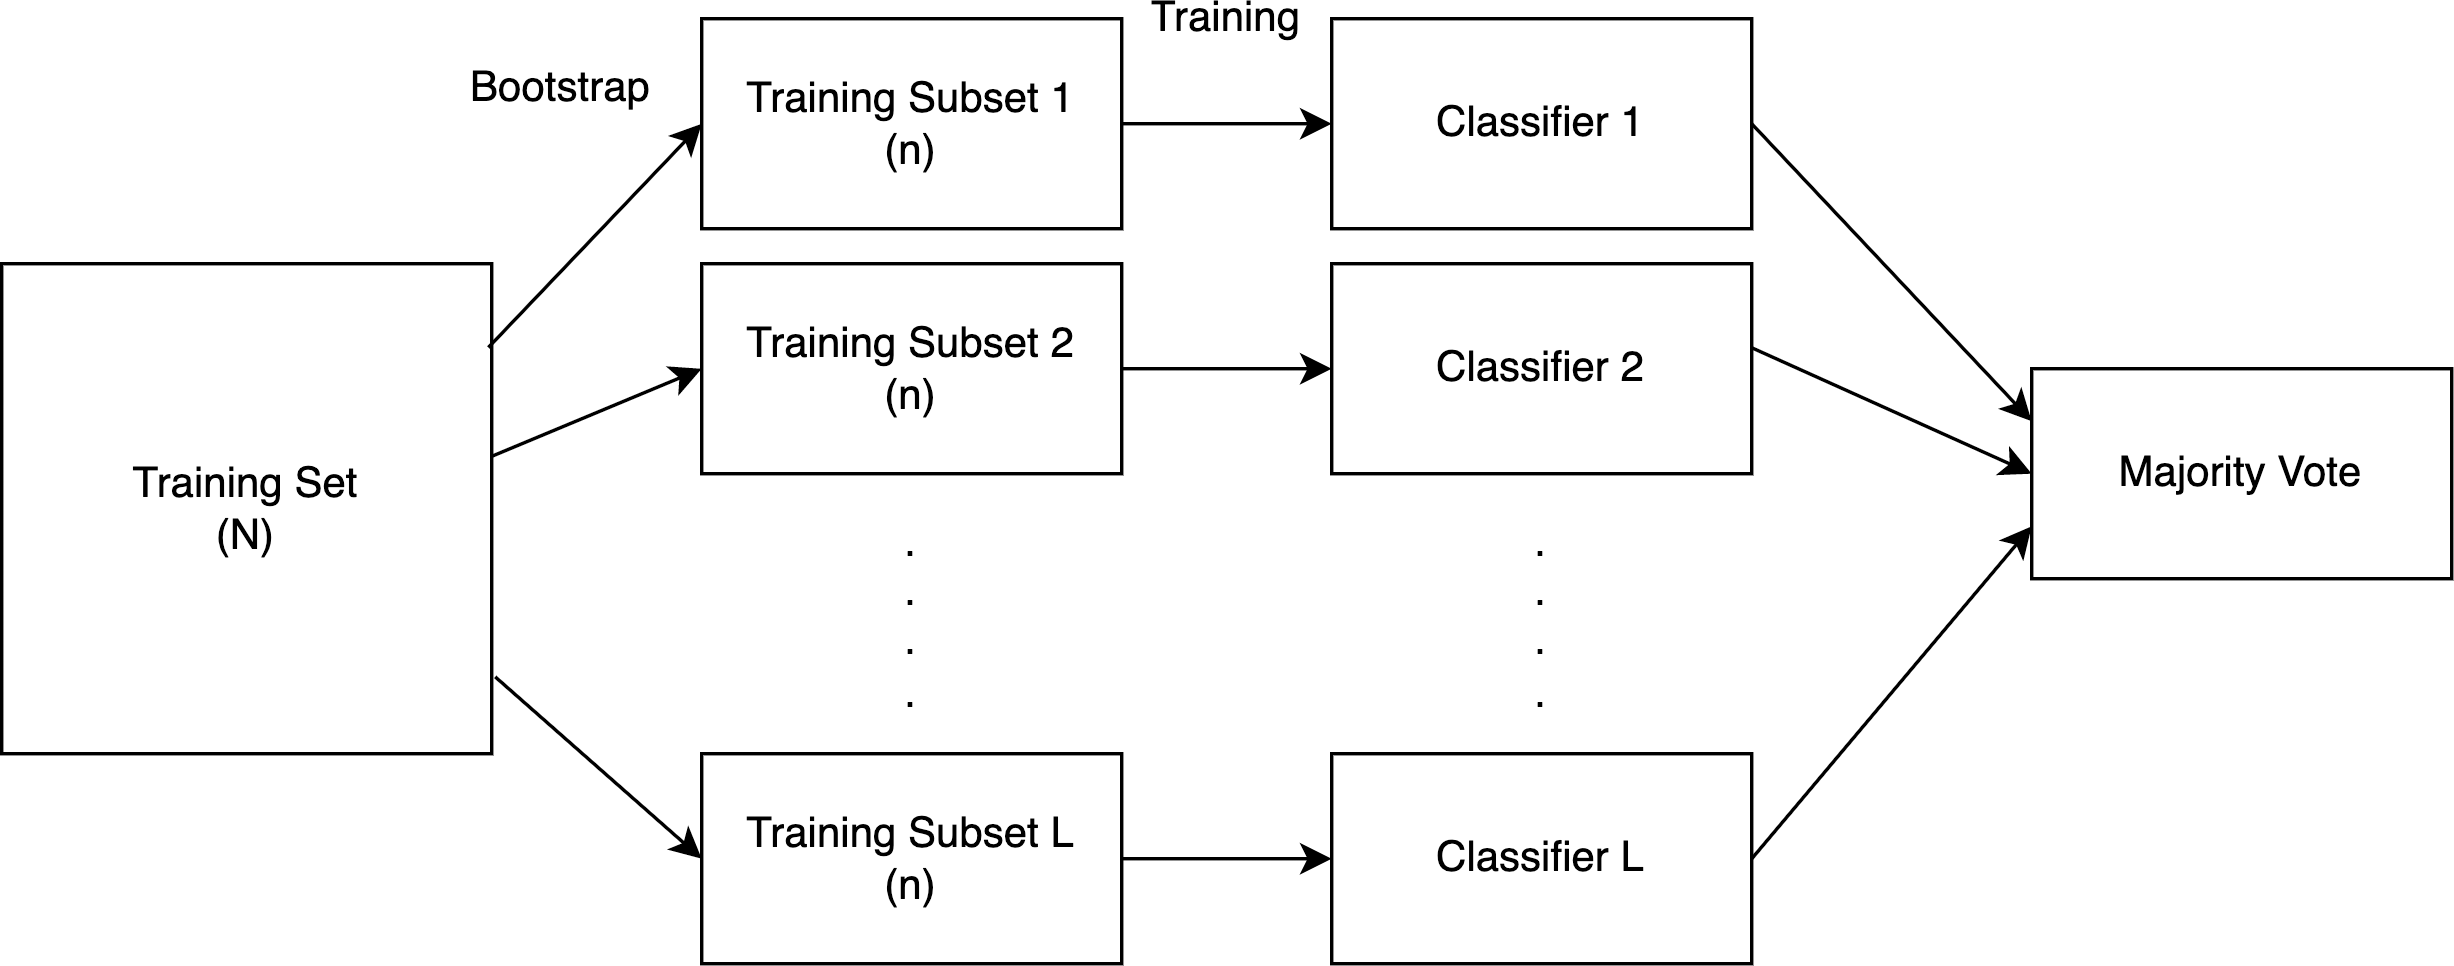
\includegraphics[width=0.85\linewidth]{gfx/m4l3_liu_fig6_bagging_procedure.png}
\par\smallskip{\small \textbf{Hình 6:} Sơ đồ biểu diễn quy trình bagging.}
\end{figure}

Chúng tôi sẽ sử dụng các mô hình với các tập con đã huấn luyện để dự báo dữ liệu kiểm định, và dự đoán cuối cùng sẽ được tạo ra từ các mô hình này thông qua bỏ phiếu đa số, như được giải thích dưới đây.

Bỏ phiếu đa số (majority vote) là phương pháp đơn giản nhất để kết hợp các bộ phân loại. Kết quả từ nhiều bộ phân loại được kết hợp bằng bỏ phiếu đa số. Đầu ra nhận được nhiều phiếu nhất sau đó được chọn làm quyết định phân loại cuối cùng (Kim \& Upneja, 2021).

\section{Thiết lập thực nghiệm}

Mục này trình bày thiết lập thực nghiệm, bao gồm chuẩn bị dữ liệu, trích xuất đặc trưng, xây dựng mô hình, và các chỉ số đánh giá.

\subsection*{Chuẩn bị dữ liệu}

Quỹ hoán đổi danh mục chỉ số SPDR S\&P 500 (SPY) đã được sử dụng trong nghiên cứu này vì đây hiện là quỹ hoán đổi danh mục (Exchange Traded Fund, ETF) S\&P 500 phổ biến nhất và là một trong những cổ phiếu có nhiều thảo luận nhất trên Stocktwits. Như được thể hiện trong Hình 7, đây là hạng mục hoạt động sôi nổi nhất trên Stocktwits vào ngày 7 tháng 9 năm 2022. Như có thể thấy, SPY có số lượng thảo luận nhiều hơn đáng kể so với bất kỳ cổ phiếu nào khác, và dựa trên quan sát của chúng tôi, SPY đã nằm trong top 3 trong một thời gian dài.

\begin{figure}[H]
\centering
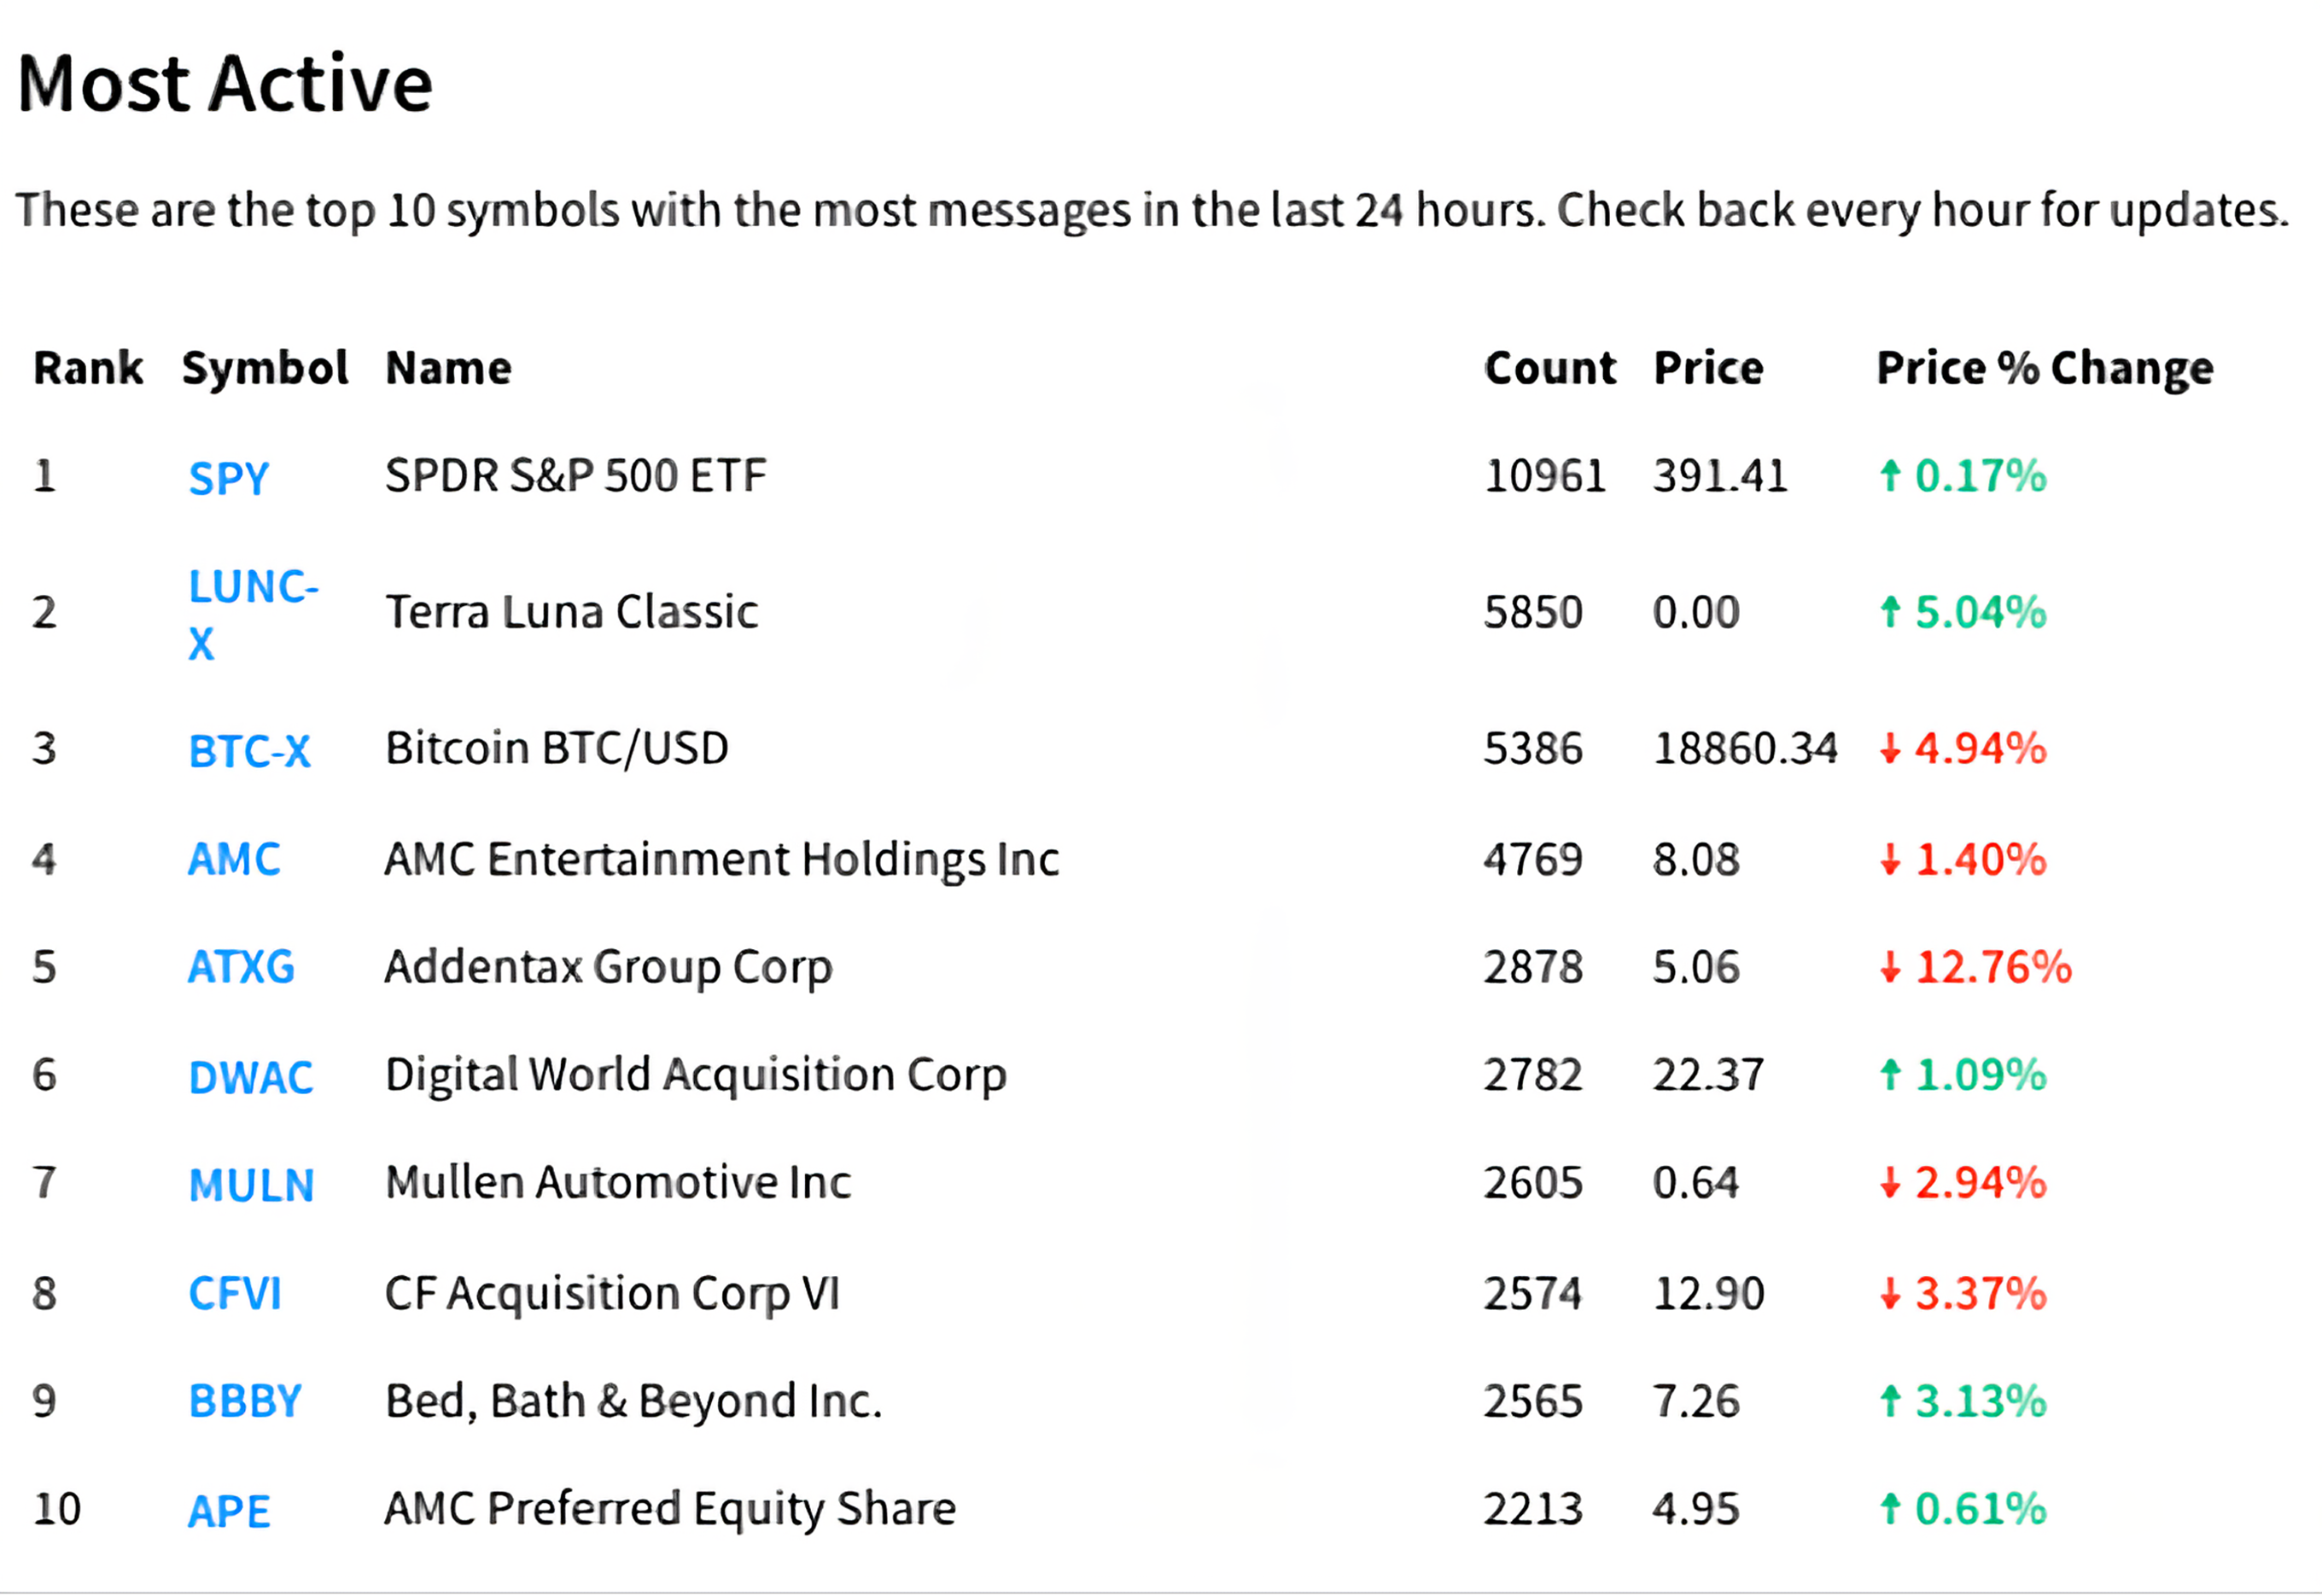
\includegraphics[width=0.85\linewidth]{gfx/m4l3_liu_fig7_top10_symbols.png}
\par\smallskip{\small \textbf{Hình 7:} Top 10 mã cổ phiếu có nhiều tin nhắn nhất vào ngày 7 tháng 9 năm 2022.}
\end{figure}

Chúng tôi thu thập tất cả bình luận về SPY và dữ liệu cổ phiếu lịch sử trên Stocktwits từ ngày 1 tháng 4 năm 2020 đến ngày 28 tháng 2 năm 2022, tổng cộng 482 ngày giao dịch, trong đó khoảng 1.33 triệu tin nhắn Stocktwits được gán nhãn và 1.73 triệu tin nhắn không được người dùng gán nhãn, với tổng số 3.06 triệu tin nhắn. Tập huấn luyện bắt đầu từ ngày 1 tháng 4 năm 2020, và giai đoạn từ ngày 5 tháng 4 năm 2021 đến ngày 28 tháng 2 năm 2022 được sử dụng làm tập kiểm định.

\subsection*{Trích xuất đặc trưng}

Chúng tôi huấn luyện mô hình bằng tổng cộng 10 đặc trưng, như được thể hiện trong Bảng 4, bao gồm ba đặc trưng cảm xúc và bảy đặc trưng được suy ra từ dữ liệu cổ phiếu lịch sử. Chúng tôi phát hiện rằng việc xem xét cả cảm xúc trước giờ mở cửa thị trường (pre-market) và cảm xúc sau giờ đóng cửa (after-market) của ngày hôm trước có thể làm tăng đáng kể độ chính xác của dự báo biến động giá cổ phiếu của chúng tôi. Điều này là do thị trường chứng khoán đặt trọng tâm đáng kể vào hai khoảng thời gian này.

Các công thức tính toán cho các đặc trưng S1 đến S3 được thể hiện trong mục con ``Tính toán chỉ số cảm xúc'' của mục trước. Để có được giá trị đặc trưng, tất cả bình luận về một cổ phiếu nhất định trên Stocktwits trong giai đoạn được chỉ định phải được thu thập và xử lý qua một mô hình phân tích cảm xúc. Sau đó, các công thức tính chỉ số cảm xúc có thể được sử dụng để tính toán các giá trị đặc trưng này. Các đặc trưng S4 đến S10 là dữ liệu cổ phiếu lịch sử và không cần tính toán.

Các đặc trưng chúng tôi đã chọn có sẵn trước khi thị trường mở cửa vào ngày dự báo, điều này cho phép chúng tôi lấy cảm xúc và đưa ra dự báo mà không bị chồng lấn. Điều này có nghĩa là kết quả dự báo sẽ có sẵn cho nhà đầu tư ngay khi thị trường mở cửa, cho phép đưa ra quyết định giao dịch sáng suốt.

\subsection*{Xây dựng mô hình}

Vì chúng tôi đang dự báo một xu hướng giá biến động (tăng hoặc giảm) thay vì giá thực tế của Quỹ hoán đổi danh mục chỉ số SPDR S\&P 500, chúng tôi phải chuyển đổi một bài toán hồi quy thành một bài toán phân loại. Vì vậy, chúng tôi cần gán nhãn dữ liệu theo phương trình dưới đây.

$$
y = \begin{cases}
1, & \text{Giá tại 12:00 EST} \geq \text{Giá mở cửa} \\
0, & \text{Giá tại 12:00 EST} < \text{Giá mở cửa}
\end{cases}
$$

\begin{figure}[H]
\centering
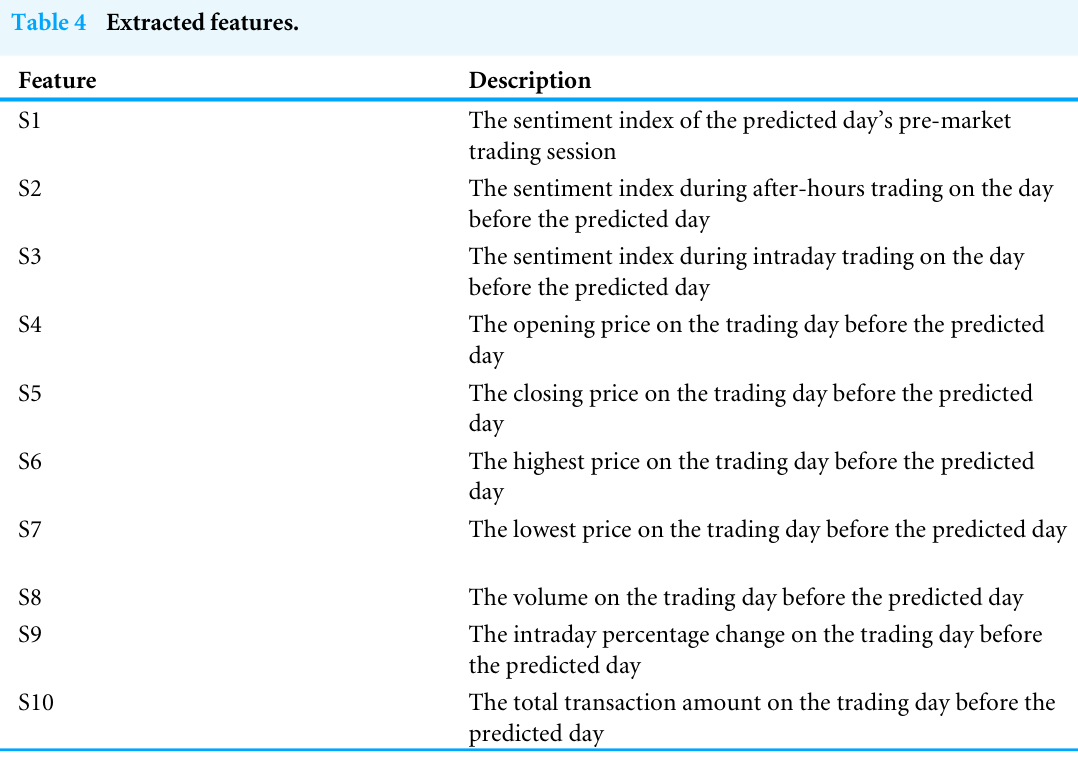
\includegraphics[width=0.95\linewidth]{gfx/m4l3_liu_table4_extracted_features.png}
\par\smallskip{\small \textbf{Bảng 4:} Các đặc trưng được trích xuất.}
\end{figure}

Chúng tôi đã sử dụng một máy vector hỗ trợ (SVM) tập hợp với bagging để xây dựng mô hình. Điều này đòi hỏi phải thiết lập các tham số cho cả bộ phân loại vector hỗ trợ (support vector classifier, SVC) và bộ phân loại bagging. SVC có một số siêu tham số quan trọng, chẳng hạn như hàm nhân, $C$ (tham số điều chuẩn hóa), và gamma (hệ số hàm nhân). Các tham số này được thể hiện chi tiết trong Bảng 5. Chúng tôi cũng đã sử dụng BaggingClassifier từ thư viện Python scikit-learn (Pedregosa và cộng sự, 2011). Bộ phân loại bagging có một số siêu tham số quan trọng cần được thiết lập, chẳng hạn như bộ ước lượng cơ sở (base estimator), số lượng bộ ước lượng (n\_estimators), và liệu các mẫu có được lấy có hoàn lại (bootstrap) hay không. Các tham số này được thể hiện chi tiết trong Bảng 6.

\begin{figure}[H]
\centering
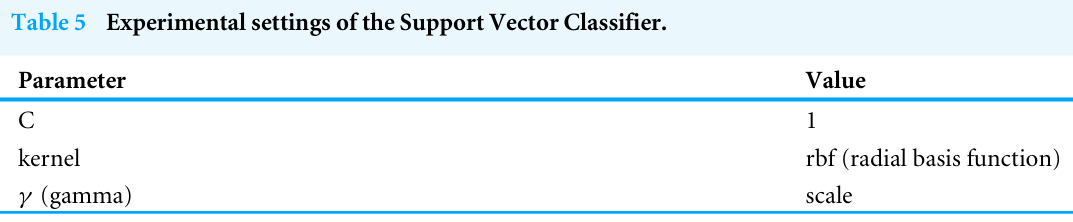
\includegraphics[width=0.8\linewidth]{gfx/m4l3_liu_table5_svc_settings.png}
\par\smallskip{\small \textbf{Bảng 5:} Thiết lập thực nghiệm của Bộ phân loại Vector Hỗ trợ (SVC).}
\end{figure}

\begin{figure}[H]
\centering
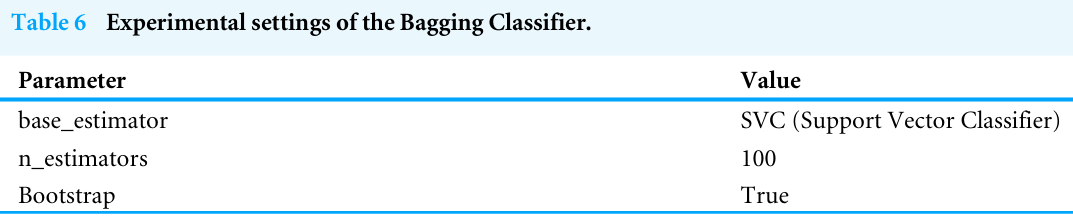
\includegraphics[width=0.8\linewidth]{gfx/m4l3_liu_table6_bagging_settings.png}
\par\smallskip{\small \textbf{Bảng 6:} Thiết lập thực nghiệm của Bộ phân loại Bagging.}
\end{figure}

\subsection*{Các chỉ số đánh giá}

Phương trình cho độ chính xác phân loại (classification accuracy) như sau, có thể biểu diễn tỷ lệ phần trăm của tổng số kết quả dự đoán đúng.

$$
\text{Accuracy} = \frac{\text{TP}+\text{TN}}{\text{TP}+\text{FP}+\text{FN}+\text{TN}}
$$

trong đó TP biểu thị giá trị dự đoán là 1 và giá trị thực cũng là 1; TN biểu thị giá trị dự đoán là 0 và giá trị thực cũng là 0; FP biểu thị giá trị dự đoán là 1 nhưng giá trị thực là 0; và FN biểu thị giá trị dự đoán là 0 nhưng giá trị thực là 1.

$$
\text{Precision} = \frac{\text{TP}}{\text{TP}+\text{FP}}
$$

trong đó độ chính xác (precision) là tỷ lệ phần trăm trong số các mẫu được dự đoán là giá cổ phiếu tăng mà giá thực tế thực sự đã tăng.

$$
\text{Recall} = \frac{\text{TP}}{\text{TP}+\text{FN}}
$$

trong đó độ bao phủ (recall) là tỷ lệ phần trăm trong số các mẫu thực tế có giá cổ phiếu tăng mà giá được dự đoán cũng tăng.

Trong việc dự đoán liệu giá cổ phiếu có tăng hay không, độ chính xác (precision) được coi là quan trọng hơn độ chính xác tổng thể (accuracy). Trong một thị trường tăng giá (bull market), cả độ chính xác (precision) và độ bao phủ (recall) đều quan trọng như nhau đối với việc ra quyết định. Tuy nhiên, trong một thị trường giảm giá (bear market), độ bao phủ (recall) trở nên quan trọng hơn độ chính xác (precision) vì nó có tác động lớn hơn đến khả năng thua lỗ tài chính tiềm ẩn (\url{http://www.bituzi.com/2019/10/confusionmatrix.html}).

$$
\text{F1 Score} = \frac{2 \cdot \text{Precision} \cdot \text{Recall}}{\text{Precision} + \text{Recall}}
$$

Điểm F1 (F1-score) ở trên là trung bình điều hòa (harmonic mean) của độ chính xác (precision) và độ bao phủ (recall). Điểm số bằng 1 đại diện cho hiệu suất cao nhất, và điểm số bằng 0 đại diện cho hiệu suất tệ nhất. Cả độ chính xác (precision) và độ bao phủ (recall) đều đóng góp như nhau vào điểm F1; do đó, điểm số càng gần 1 thì mô hình càng tốt (\url{https://scikit-learn.org/stable/modules/generated/sklearn.metrics.f1_score.html}). Do đó, đối với chủ đề này, chúng tôi đánh giá các phương pháp bằng điểm F1.

\section{Kết quả}

Trong nghiên cứu này, chúng tôi đã tiến hành năm thực nghiệm để đo lường hiệu suất của việc kết hợp các chỉ số cảm xúc trong dự đoán biến động giá cổ phiếu. Ngoài ra, thông qua các thực nghiệm này, chúng tôi có thể xác định liệu việc bổ sung cảm xúc có giúp mô hình dự báo biến động giá cổ phiếu hay không và so sánh hiệu suất của các phương pháp khác nhau để thu thập chỉ số cảm xúc. Các thực nghiệm (viết tắt là TN) như sau:
\begin{itemize}
  \item \textbf{TN 1.} Trong việc xây dựng mô hình, chỉ dữ liệu cổ phiếu lịch sử được sử dụng làm đặc trưng và không có dữ liệu cảm xúc nào được đưa vào xem xét. Do đó, chỉ các đặc trưng S4 đến S10 trong Bảng 4 được sử dụng trong mô hình.
  \item \textbf{TN 2.} Ngoài việc sử dụng dữ liệu cổ phiếu lịch sử, chúng tôi bổ sung các chỉ số cảm xúc được tính toán từ dữ liệu cảm xúc do người dùng cung cấp làm đặc trưng.
  \item \textbf{TN 3.} Để tăng tổng số lượng cảm xúc, không chỉ cảm xúc do người dùng cung cấp mà cả các bình luận không được gán nhãn cũng được phân loại là tăng giá hoặc giảm giá bằng một mô hình phân tích cảm xúc hai lớp. Chúng tôi sử dụng mô hình phân tích cảm xúc roberta-base-Stocktwits-finetuned (\url{https://huggingface.co/zhayunduo/roberta-base-Stocktwits-finetuned}) trong thực nghiệm này, đây là một mô hình phân tích cảm xúc được huấn luyện trên các bình luận Stocktwits và có thể đưa ra kết quả tăng giá hoặc giảm giá với độ chính xác 93.43\%.
  \item \textbf{TN 4.} Tất cả bình luận được gán nhãn bằng mô hình FinBERT, và các chỉ số cảm xúc được tính toán làm đặc trưng.
  \item \textbf{TN 5.} Tất cả bình luận được gán nhãn bằng mô hình VADER, và các chỉ số cảm xúc được tính toán làm đặc trưng, giống cách Koukaras, Nousi \& Tjortjis (2022) làm trong thực nghiệm tương tự với VADER. Mô hình cũng đưa ra ba lớp kết quả.
\end{itemize}

Theo Ren, Wu \& Liu (2019), việc lựa chọn ngẫu nhiên tập huấn luyện và tập kiểm định trong bộ dữ liệu của chúng tôi có thể dẫn đến thiên lệch nhìn trước. Ví dụ, chúng tôi dự đoán biến động giá cổ phiếu của ngày hôm nay, nhưng tập huấn luyện của chúng tôi chứa dữ liệu từ ngày mai và ngày kia, mang lại cho mô hình phân loại một lợi thế trước về xu hướng tương lai mà không thể đạt được trong các ứng dụng thực tế. Chúng tôi giải quyết vấn đề thiên lệch nhìn trước bằng cách sử dụng phương pháp cửa sổ trượt. Hình 8 minh họa ý tưởng này một cách đầy đủ. Để bắt đầu, cần xác định kích thước cửa sổ trượt phù hợp nhất cho mỗi thực nghiệm. Kích thước được xác định bằng cách huấn luyện trên các ngày trước đó, dự báo biến động của ngày tiếp theo cho đến cuối bộ dữ liệu, và chọn kích thước cửa sổ có độ chính xác cao nhất cho thực nghiệm. Khi chúng tôi đã chọn được kích thước tối ưu cho cửa sổ trượt, chúng tôi có thể sử dụng kích thước này vào tương lai để dự báo biến động giá của ngày mới. Kết quả là, chúng tôi huấn luyện và kiểm định mô hình bằng phương pháp cửa sổ trượt, cho phép chúng tôi tránh hiệu quả vấn đề thiên lệch nhìn trước và ngăn mô hình quá khớp với dữ liệu.

\begin{figure}[H]
\centering
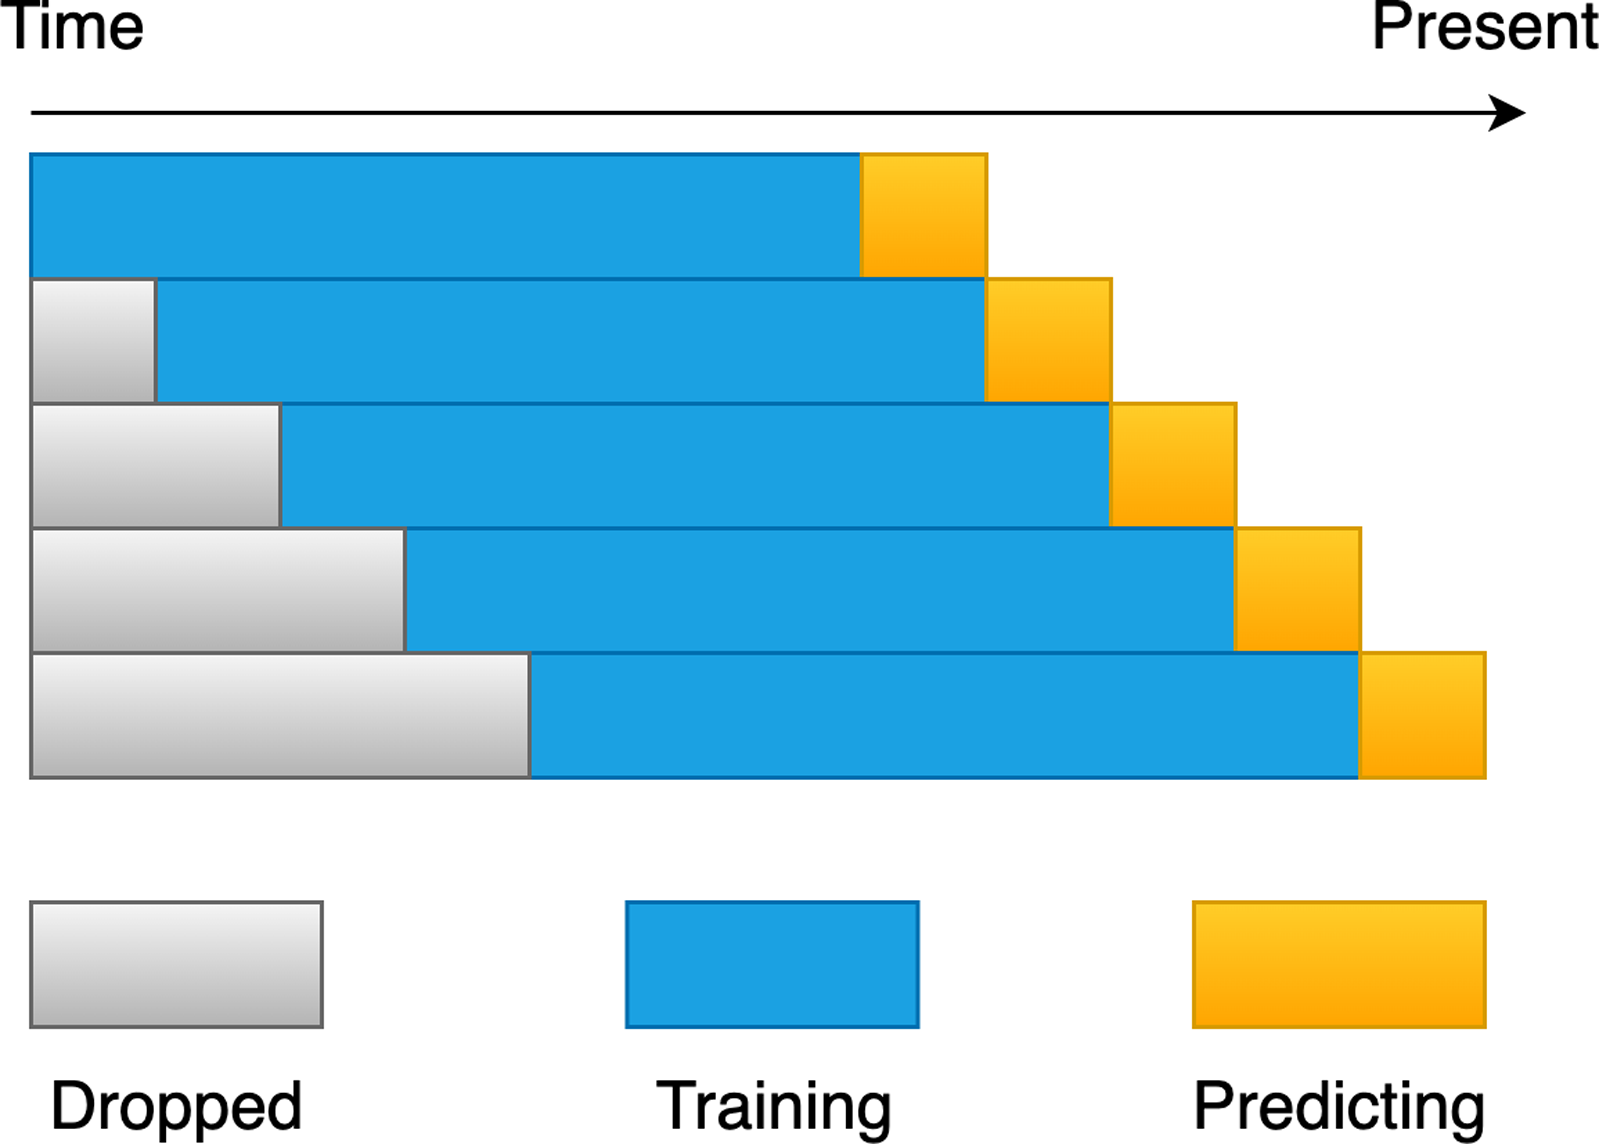
\includegraphics[width=0.6\linewidth]{gfx/m4l3_liu_fig8_rolling_window_procedure.png}
\par\smallskip{\small \textbf{Hình 8:} Sơ đồ biểu diễn quy trình cửa sổ trượt (rolling window).}
\end{figure}

Ngoài ra, chúng tôi tin rằng kích thước của cửa sổ trượt không nên quá nhỏ, vì điều kiện thị trường có thể thay đổi trong ngắn hạn. Ví dụ, nếu thị trường hiện đang tăng giá, một số yếu tố hoặc tin tức thị trường có thể khiến nó chuyển sang giảm giá. Nếu dữ liệu dùng để huấn luyện mô hình không đủ, ngay cả khi kết quả dự đoán tốt, khả năng tổng quát hóa của mô hình có thể kém hơn. Do đó, mặc dù bộ dữ liệu cho nghiên cứu này bị giới hạn, chúng tôi đặt kích thước huấn luyện của cửa sổ trượt trong khoảng từ 232 đến 252 (tương đương số ngày làm việc trong khoảng một năm), kích thước kiểm định của một cửa sổ là 1 cho mục đích thực nghiệm và phân tích, và kích thước cửa sổ huấn luyện được đặt là một số chia hết cho 2. Vì vậy, chúng tôi huấn luyện 11 mô hình dự đoán với các kích thước cửa sổ huấn luyện khác nhau trong mỗi thực nghiệm. Hơn nữa, do các điều kiện thị trường khác nhau giữa thị trường tăng giá và giảm giá, tập dữ liệu huấn luyện có thể mất cân bằng. Do đó, chúng tôi sử dụng SMOTE (Chawla và cộng sự, 2002), một kỹ thuật lấy mẫu quá mức (oversampling), để cân bằng dữ liệu huấn luyện.

Điểm F1 tốt nhất thu được từ kết quả thực nghiệm được trình bày trong Bảng 7.

\begin{figure}[H]
\centering
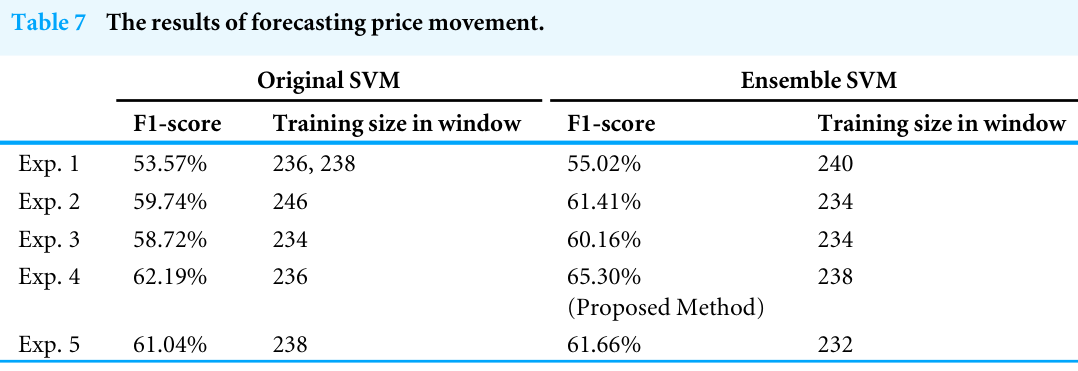
\includegraphics[width=0.95\linewidth]{gfx/m4l3_liu_table7_forecasting_results.png}
\par\smallskip{\small \textbf{Bảng 7:} Kết quả dự báo biến động giá.}
\end{figure}

Trong TN 1, việc thiếu các chỉ số cảm xúc dẫn đến kết quả kém chính xác hơn so với các thực nghiệm khác. Do đó, chúng tôi sử dụng kết quả của TN 1 làm cơ sở (baseline) cho các thực nghiệm còn lại.

Trong TN 2, việc bổ sung các cảm xúc được chủ động chỉ ra bởi người dùng cải thiện đáng kể hiệu suất của các dự đoán biến động giá cổ phiếu. Điều này chứng minh một mối tương quan mạnh mẽ giữa cảm xúc nhà đầu tư và biến động giá cổ phiếu.

Trong TN 3, chúng tôi đã sử dụng một mô hình phân tích cảm xúc hai lớp để tăng tổng lượng cảm xúc trong phân tích của chúng tôi. Tuy nhiên, chúng tôi phát hiện rằng một số bình luận không được gán nhãn liên quan đến chỉ trích về chính trị hoặc hoạt động của nền tảng. Những bình luận này không phù hợp để phân loại là tăng giá hoặc giảm giá, nhưng mô hình vẫn gán một nhãn do hạn chế của nó chỉ có thể đưa ra hai loại cảm xúc. Kết quả là, điểm F1 của dự báo giá cổ phiếu thấp hơn so với TN 2. Để khảo sát sâu hơn vấn đề này, chúng tôi đã chọn ngẫu nhiên 100 bình luận chưa được gán nhãn để gán nhãn thủ công và phát hiện rằng 45 trong số đó không phù hợp để được gán nhãn là tăng giá hoặc giảm giá. Những kết quả này chứng minh rằng việc sử dụng một mô hình phân tích cảm xúc hai lớp để thu thập thêm cảm xúc không nhất thiết cải thiện điểm F1 so với việc chỉ sử dụng các cảm xúc hai lớp do người dùng chủ động gán nhãn.

Trong TN 4, chúng tôi đã thu thập tất cả các bình luận về SPY trên Stocktwits trong hai năm qua và phân loại chúng bằng mô hình FinBERT, mô hình này cung cấp không chỉ cảm xúc tích cực và tiêu cực mà còn cả cảm xúc trung lập. Điều này giải quyết vấn đề của TN 3, nơi một mô hình phân tích cảm xúc hai lớp có thể phân loại một số bình luận không tăng giá và không giảm giá là tăng giá hoặc giảm giá. Tuy nhiên, FinBERT có khả năng phân loại các cảm xúc không liên quan đến tài chính là trung lập. Bằng cách tính toán công thức của chỉ số cảm xúc ba lớp được đề cập trong mục ``Phương pháp luận'', chúng tôi có thể phân biệt các bình luận không tăng giá hoặc không giảm giá về các chủ đề không liên quan đến tài chính, và các chỉ số cảm xúc hợp lý được thu được. Điểm F1 của phương pháp thay thế được đề xuất cao hơn các phương pháp khác.

Trong TN 5, chúng tôi đã sử dụng VADER làm mô hình phân tích cảm xúc, có khả năng đưa ra ba kết quả (tích cực, tiêu cực, và trung lập). Tuy nhiên, vì mô hình này không được thiết kế chuyên biệt cho lĩnh vực tài chính, hiệu suất của nó không vượt qua TN 4 (FinBERT).

\section{Thảo luận}

Hình 9 trình bày các biểu đồ tần suất điểm F1 (F1-score frequency histograms) cho mỗi thực nghiệm. Các biểu đồ cho thấy SVM tập hợp được triển khai cải thiện hiệu suất dự đoán biến động cổ phiếu trong tất cả các thực nghiệm. Bằng cách sử dụng kỹ thuật bagging, SVM tập hợp trong nghiên cứu này kết hợp các dự đoán từ nhiều bộ dự báo cơ sở, nắm bắt hiệu quả tính đa dạng của tập dữ liệu và nâng cao khả năng tổng quát hóa của mô hình. Cách tiếp cận này cũng giảm khả năng quá khớp so với việc sử dụng một bộ dự báo đơn lẻ, từ đó nâng cao độ chính xác. Kết quả tối ưu đạt được bằng phương pháp luận được đề xuất, sử dụng FinBERT để phân tích cảm xúc và SVM tập hợp cho dự đoán biến động giá cổ phiếu trong TN 4, đạt điểm F1 đỉnh là 65.30\%.

\begin{figure}[H]
\centering
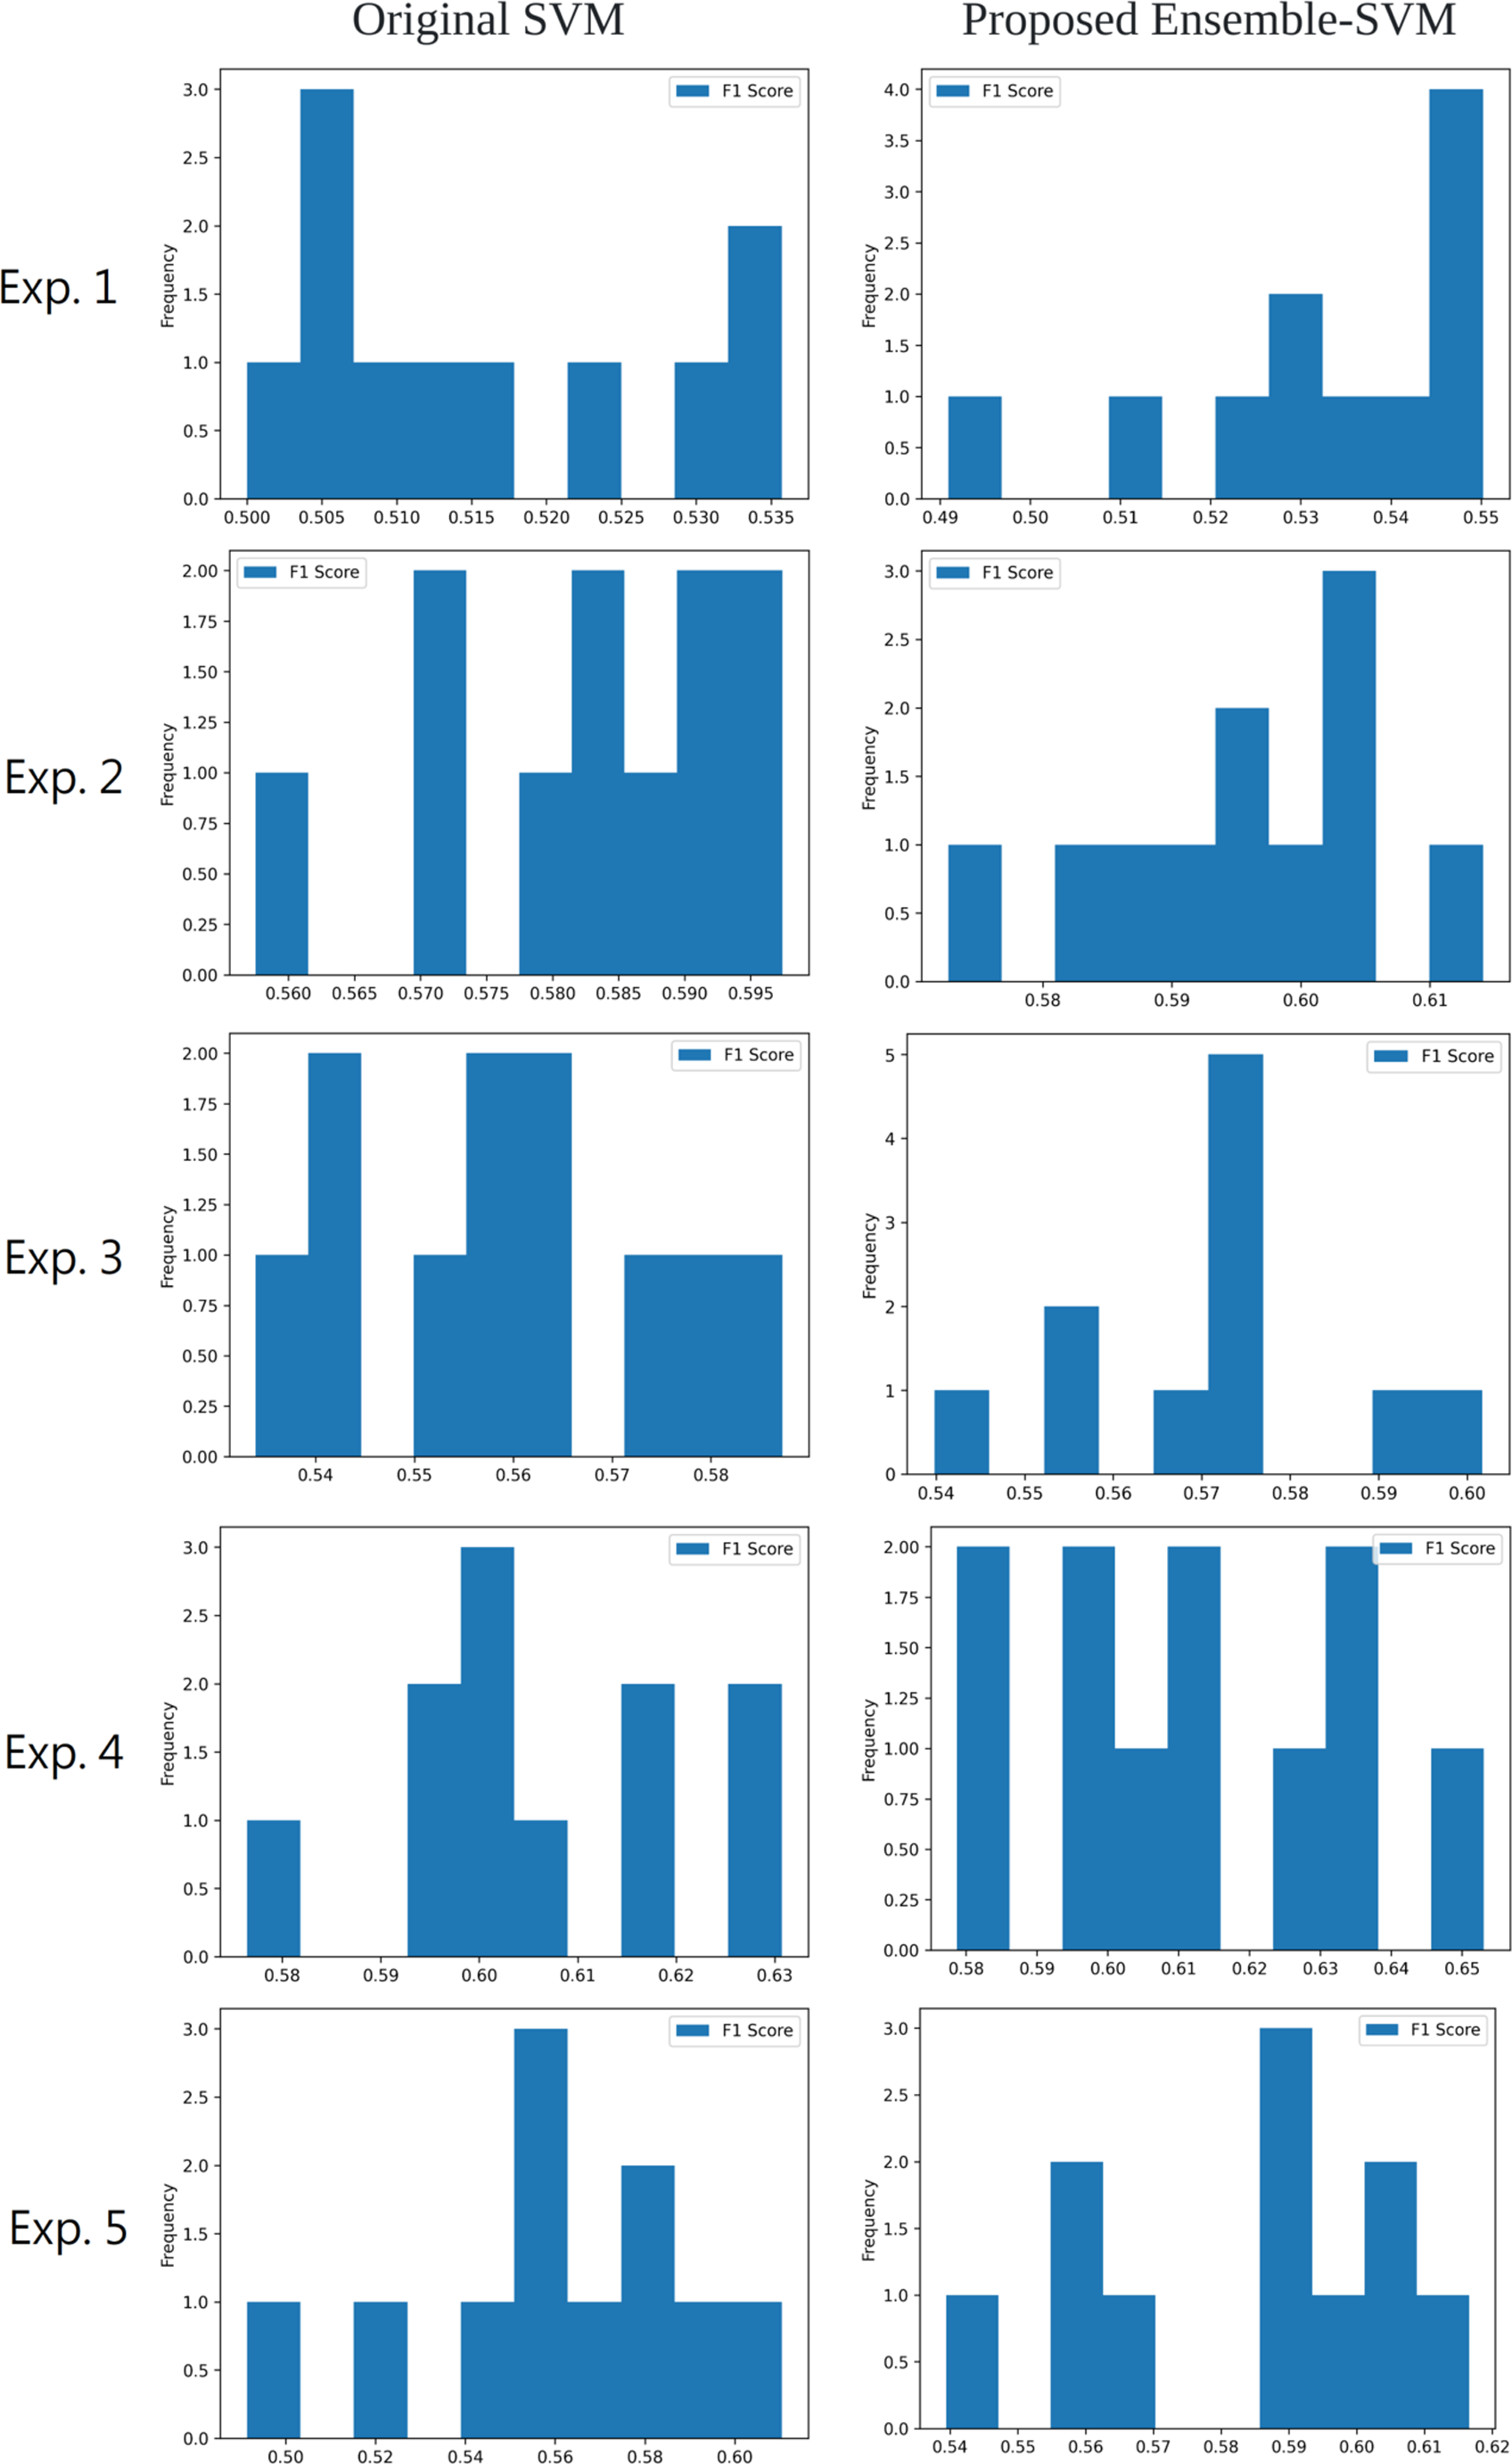
\includegraphics[width=0.85\linewidth]{gfx/m4l3_liu_fig9_f1score_histogram.png}
\par\smallskip{\small \textbf{Hình 9:} Biểu đồ tần suất của điểm F1 cho mỗi thực nghiệm.}
\end{figure}

Trong TN 1 và TN 2, chúng tôi so sánh mức cải thiện điểm F1 của dự đoán biến động giá cổ phiếu khi bổ sung cảm xúc nhà đầu tư. Vì Gupta \& Chen (2020) đã phát triển nhiều bộ phân tích cảm xúc hai lớp với độ chính xác khoảng 75 đến 85\%, và phân tích cảm xúc được theo sau bởi dự đoán biến động giá cổ phiếu, kết quả cho thấy nhiều bình luận hơn có hiệu quả trong việc cải thiện độ chính xác. Do đó, để so sánh với phương pháp này, chúng tôi đã sử dụng một bộ phân tích cảm xúc hai lớp với độ chính xác 93\% trong TN 3. Tuy nhiên, kết quả của dự đoán biến động giá cổ phiếu không đạt yêu cầu. Gupta \& Chen (2020) đề cập rằng một mô hình có cảm xúc trung lập có thể giảm nhiễu và cải thiện độ chính xác. Do đó, trong phương pháp của Koukaras, Nousi \& Tjortjis (2022), một mô hình có cảm xúc trung lập như VADER đã được sử dụng để phân tích, và kết quả tốt đã đạt được. Tuy nhiên, vì họ chỉ sử dụng 22 ngày trong tập kiểm định, chúng tôi không thể xác định khả năng tổng quát hóa của nó. Trong TN 5, chúng tôi đã sử dụng bộ dữ liệu của mình, lớn gấp hơn 10 lần so với bộ dữ liệu của họ, để dự đoán. Kết quả cho thấy cách tiếp cận này vượt trội hơn TN 3, nhưng không nhất thiết tốt hơn TN 2 (chỉ dự đoán dựa trên cảm xúc do người dùng chủ động gán nhãn). Trong TN 4, chúng tôi đề xuất một cách tiếp cận thay thế, đó là áp dụng mô hình FinBERT làm mô hình phân tích cảm xúc. Kết quả cho thấy cách tiếp cận này đạt được kết quả thực nghiệm tốt nhất.

\section{Kết luận}

Trong bài báo này, chúng tôi đề xuất một cách tiếp cận thay thế cho phân tích cảm xúc của bình luận Stocktwits nhằm dự đoán biến động giá cổ phiếu. Phương pháp được đề xuất của chúng tôi sử dụng mô hình FinBERT để giảm nhiễu, nâng cao mức độ vĩ mô và độ chính xác của các chỉ số cảm xúc, và giải quyết các lỗi phân loại phát sinh từ mô hình phân tích cảm xúc hai lớp. Bằng cách so sánh phương pháp của chúng tôi với các kỹ thuật được sử dụng trong các nghiên cứu trước đây, chúng tôi chứng minh tính hiệu quả của nó. Hơn nữa, chúng tôi giới thiệu một mô hình máy vector hỗ trợ tập hợp để cải thiện khả năng tổng quát hóa và tăng độ chính xác của các dự đoán biến động giá cổ phiếu. Chúng tôi cũng áp dụng phương pháp cửa sổ trượt để ngăn thiên lệch nhìn trước. Nhìn chung, nghiên cứu của chúng tôi đóng góp vào khối lượng nghiên cứu ngày càng tăng về dự đoán giá cổ phiếu dựa trên cảm xúc và có tiềm năng hỗ trợ nhà đầu tư đưa ra các quyết định sáng suốt.

Mặc dù đạt được độ chính xác lý tưởng trong việc dự đoán biến động giá cổ phiếu bằng phương pháp được đề xuất, vẫn còn những hạn chế khi chỉ dựa vào cảm xúc. Có thể xác định hai hướng chính để cải thiện trong tương lai. Thứ nhất, các phương pháp chỉ dựa vào cảm xúc mạng xã hội để dự đoán giá cổ phiếu dễ bị tổn thương trước sự thao túng có chủ đích, chẳng hạn như sự kiện ép bán khống (short squeeze) của GameStop năm 2021. Do đó, cần thiết phải thiết lập các cơ chế bảo vệ chống lại các thao túng như vậy trong tương lai. Thứ hai, hiệu suất của các phương pháp chỉ phụ thuộc vào cảm xúc mạng xã hội để dự đoán giá cổ phiếu là có giới hạn. Để nâng cao độ chính xác của dự đoán, chúng tôi dự định kết hợp phương pháp được đề xuất trong bài báo này với các chỉ báo phân tích kỹ thuật trong các nghiên cứu tương lai.

\section{Thông tin bổ sung và các công bố}

\subsection*{Tài trợ}

Nghiên cứu này được tài trợ bởi Chương trình Nghiên cứu Chung giữa Viện Công nghệ Kyushu và Đại học Khoa học và Công nghệ Quốc gia Đài Loan, theo khoản tài trợ Kyutech-NTUST-109-03. Bên tài trợ không có vai trò gì trong việc thiết kế nghiên cứu, thu thập và phân tích dữ liệu, quyết định công bố, hay việc chuẩn bị bản thảo.

\subsection*{Công bố tài trợ}

Các tác giả đã công bố thông tin tài trợ sau đây: Chương trình Nghiên cứu Chung giữa Viện Công nghệ Kyushu và Đại học Khoa học và Công nghệ Quốc gia Đài Loan: Kyutech-NTUST-109-03.

\subsection*{Xung đột lợi ích}

Các tác giả tuyên bố không có xung đột lợi ích nào.

\subsection*{Đóng góp của các tác giả}

\begin{itemize}
  \item Jin-Xian Liu đã hình thành và thiết kế các thí nghiệm, thực hiện các thí nghiệm, phân tích dữ liệu, thực hiện công việc tính toán, chuẩn bị các hình và/hoặc bảng, viết hoặc rà soát các bản thảo của bài báo, và phê duyệt bản thảo cuối cùng.
  \item Jenq-Shiou Leu đã hình thành và thiết kế các thí nghiệm, phân tích dữ liệu, viết hoặc rà soát các bản thảo của bài báo, và phê duyệt bản thảo cuối cùng.
  \item Stefan Holst đã hình thành và thiết kế các thí nghiệm, phân tích dữ liệu, viết hoặc rà soát các bản thảo của bài báo, và phê duyệt bản thảo cuối cùng.
\end{itemize}

\subsection*{Khả năng tiếp cận dữ liệu}

Dữ liệu phân tích cảm xúc, dữ liệu thực nghiệm, và dữ liệu lịch sử giá cổ phiếu được cung cấp trong các Tệp Bổ sung (Supplemental Files). Bộ dữ liệu tin nhắn SPY có sẵn tại Figshare: Liu, Jin-Xian (2022): SPY\_stocktwits\_messages.csv. figshare. Dataset. \url{https://doi.org/10.6084/m9.figshare.20237736.v1}.

\subsection*{Thông tin bổ sung}

Thông tin bổ sung cho bài báo này có thể được tìm thấy trực tuyến tại \url{http://dx.doi.org/10.7717/peerj-cs.1403#supplemental-information}.

% [Đã lược bỏ danh mục Tài liệu tham khảo gốc (tiếng Anh, trích dẫn của tác giả bài gốc) để giảm dung lượng chương; không ảnh hưởng nội dung học thuật chính.]
